\documentclass[review]{elsarticle}
\usepackage{lineno,hyperref}
\modulolinenumbers[5]
\journal{Environmental Modelling \& Software}
\bibliographystyle{elsarticle-num}
%%%

%%% General usepackages, definitions, etc.
\usepackage[acronym,toc]{glossaries}
\usepackage{graphicx}
\usepackage{booktabs} % nice rules for tables
\usepackage{microtype} % if using PDF
\usepackage{hyperref}
\usepackage{amsmath}
\usepackage{moreverb} % for verbatim snippets of code
\usepackage{fancyvrb}
\usepackage{tabularx} % for tables with line breaks
\usepackage{threeparttable} % for tables with notes
\usepackage[capitalize, noabbrev]{cleveref} % for reference multiple figures
\usepackage{calc} % allows for arithmetic on latex variables
\usepackage{algorithm2e} % for algorithms
\usepackage{multirow} % combining rows in tables
\usepackage{footnote}
\usepackage{titlesec} % for using \titleformat
\usepackage{fixltx2e} % for using \textsubscript
\usepackage{bashful}
\usepackage{xspace}
\usepackage{color}
\usepackage{subfig}
\usepackage{minted}
%%%%% 

%%%%% Helpers

\newcommand{\code}[1]{\lstinline[basicstyle=\ttfamily\color{black}]|#1|}
\newcommand{\codeb}[1]{\texttt{#1}}
\newcommand{\units}[1] {\:\text{#1}}%
\newcommand{\TODO}[1]{\textbf{TODO: #1}}

%%% gases
\newcommand{\cotwo}{CO\textsubscript{2}~}
\newcommand{\nox}{NO\textsubscript{x}}
\newcommand{\noxx}{NO\textsubscript{x}~}
\newcommand{\nht}{NH\textsubscript{3}}
\newcommand{\nhtt}{NH\textsubscript{3}~}


\makeatletter
\newcommand\footnoteref[1]{\protected@xdef\@thefnmark{\ref{#1}}\@footnotemark}
\makeatother


%%% Figure path
\graphicspath{{./figs/}}

%%% Plural gls entries
\newacronym[
  \glslongpluralkey={Integrated Assessment Models},
  \glsshortpluralkey={IAMs}
]{iam}{IAM}{Integrated Assessment Model}
\newacronym[
  \glslongpluralkey={Shared Socioeconomic Pathways},
  \glsshortpluralkey={SSPs}
]{ssp}{SSP}{Shared Socioeconomic Pathway}
\newacronym[
  \glslongpluralkey={Representative Concentration Pathways},
  \glsshortpluralkey={RCPs}
]{rcp}{RCP}{Representative Concentration Pathway}
\newacronym[
  \glslongpluralkey={Greenhouse Gases},
  \glsshortpluralkey={GHGs}
]{ghg}{GHG}{Greenhouse Gas}


%%% Acronyms
\newacronym{sres}{SRES}{Special Report on Emissions Scenarios}
\newacronym{cmip6}{CMIP6}{Coupled Model Intercomparison Project (Phase 6)}
\newacronym{smip}{ScenarioMIP}{Scenario Model Intercomparison Project}
\newacronym{ceds}{CEDS}{Community Emissions Data System}
\newacronym{esm}{ESM}{Earth System Model}
\newacronym{luc}{LUC}{Land-use Change}
\newacronym{luluc}{LULUC}{Land-use and Land-use Change}
\newacronym{weu}{WEU}{Western Europe}
\newacronym{nam}{NAM}{North America}
\newacronym{pao}{PAO}{Pacific OECD}
\newacronym{eeu}{EEU}{Central and Eastern Europe}
\newacronym{fsu}{FSU}{Former Soviet Union}
\newacronym{pas}{PAS}{Other Pacific Asia}
\newacronym{cpa}{CPA}{Centrally-planned Asia and China}
\newacronym{sas}{SAS}{South Asia}
\newacronym{mea}{MEA}{Middle East and North Africa}
\newacronym{afr}{AFR}{Sub-Saharan Africa}
\newacronym{lam}{LAM}{Latin America and the Caribbean}
\newacronym{cli}{CLI}{Command Line Interface}
\newacronym{wmo}{WMO}{World Meteorological Organization}

\makeglossaries


\begin{document}

%%% ELS input
\begin{frontmatter}

\title{A Methodology and Implementation of Automated Emissions Harmonization for Use in Integrated Assessment Models}

%% Group authors per affiliation:
\author[iiasa]{Matthew J. Gidden\corref{corref}}
\ead{gidden@iiasa.ac.at}
\cortext[corref]{Corresponding author}

\author[nies]{Shinichiro Fujimori}
\author[pbl]{Maarten van den Berg}
\author[pik]{David Klein}
\author[pnnl]{Steven J. Smith}
\author[pbl]{Detlef P. van Vuuren}
\author[iiasa]{Keywan Riahi}

\address[iiasa]{International Institute for Applied Systems Analysis,
  Schlossplatz 1, A-2361 Laxenburg, Austria}
\address[nies]{Center for Social and Environmental Systems Research, National Institute for Environmental Studies, 16-2 Onogawa, Tsukuba, Ibaraki 305-8506, Japan}
\address[pbl]{PBL Netherlands Environmental Assessment Agency, Postbus 30314, 2500 GH The Hague, Netherlands}
\address[pik]{Potsdam Institute for Climate Impact Research (PIK), Member of the Leibniz Association, P.O. Box 60 12 03, D-14412 Potsdam, Germany}
\address[pnnl]{Joint Global Change Research Institute, 5825 University Research Court, Suite 3500, College Park, MD 20740}

\begin{abstract}
Emissions harmonization refers to the process used to match greenhouse gas (GHG)
and air pollutant results from Integrated Assessment Models (IAMs) against a
common source of historical emissions. To date, harmonization has been performed
separately by individual modeling teams. For the hand-over of emission data for
the Shared Socioeconomic Pathways (SSPs) to climate model groups, a new
automated approach based on commonly agreed upon algorithms was developed. This
work describes the novel methodology for determining such harmonization methods
and an open-source Python software library implementing the methodology. Results
are shown for two example scenarios (with and without climate policy cases)
using the IAM MESSAGE-GLOBIOM that satisfactorily harmonize over 96\% of the
total emissions trajectories while having a negligible effect on key long-term
climate indicators. This new capability enhances the comparability across
different models, increases transparency and robustness of results, and allows
other teams to easily participate in intercomparison exercises by using the
same, openly available harmonization mechanism.
\end{abstract}

\begin{keyword}
Integrated Assessment Models, Harmonization, Greenhouse Gases (GHGs), Air Pollution 
\end{keyword}

\end{frontmatter}

\linenumbers

%%%
%%%%%%%%%%%%%%%%%%%%%%%%%%%%%%%%%%%%%%%%%%%%%%%%%%%%%%%%%%%%%%%%%%%%%%%%%%%%%%%%
\newpage
\section*{Software Availability}

\texttt{aneris}, first made available in 2017, is available online at
\url{https://github.com/gidden/aneris} as a free and open-source Python software
library (approximately 2000 lines of code). The \texttt{aneris} software was
developed by the lead author, Matthew J. Gidden, Ph.D., whose contact
information is shown on the title page of this manuscript. Documentation for the
\texttt{aneris} Python package, including software requirements, is available
\href{http://mattgidden.com/aneris/}{online}.

\newpage

\section{Introduction}

\glspl{iam} are tools used to understand the complex interactions between
energy, economy, land use, water, and climate systems. \glspl{iam} provide
global projections of systemic change by dividing the world into a number of
representative regions (typically 10 to 30), the definition of which is distinct
for each model \cite{krey_global_2014}. Results from \glspl{iam} are integral in
a number of international studies, which notably include projections of climate
and economic futures. Recently, the \gls{iam} community has developed scenarios
based on the \glspl{ssp} \cite{van_vuuren_energy_2017, fricko_marker_2017,
  fujimori_ssp3:_2017, calvin_ssp4:_2017, kriegler_fossil-fueled_2017} which
quantify a variety of potential global futures. The \glspl{ssp} are designed to
be used in research that include \gls{esm} simulations, climate impact,
adaptation and climate mitigation studies \cite{vuuren_new_2013}.

While \glspl{iam} are implemented in myriad ways, including simulation and
optimization, the core inputs and outputs are similar across different
models. Modeling teams incorporate data on energy systems, land use, economics,
demographics and emissions sources and concentrations, among other data, in
order to provide consistent existing trajectories of modeled variables. The
models then provide estimates of future trajectories of these variables under
various socio-economic and technological assumptions as well as proposed policy
constraints, e.g., targets for future \gls{ghg} emissions.

The emissions trajectories calculated by \glspl{iam} are critical inputs for
ongoing, worldwide scientific community efforts in the \gls{cmip6}
\cite{eyring_overview_2016}, which is utilizing a number of marker \gls{ssp} scenarios
developed by the \gls{iam} community (\gls{smip})
\cite{oneill_scenario_2016}. These trajectories are endogenously calculated by
modeling the individual technologies and sectors that contribute towards the
emissions of different air pollutants and \glspl{ghg} as well as various
mitigation technologies. However, the historical emissions starting points of
models can differ by large amounts depending on the region, sector, and
emissions species.

In practice, \glspl{iam} calculate the total source intensity of emitting
technologies, for example the total activity of coal power plants in China, and
incorporate emissions-intensity factors for individual gas species, for example
the quantity of sulfur emissions from coal plants per megawatt-hour of
production. Models are generally \textit{calibrated} to historical data sources
in one or more base years. Results in the historical period may differ between
models as a result of the sometimes large uncertainties in historical data
sets. Models can also differ in their choice of base-year, which may lag behind
available inventory data. In addition, models have varying sectoral, regional,
and fuel aggregations.

The global climate change community has recently developed a new global
historical emissions data set for both anthropogenic emissions (i.e., the
\gls{ceds} \cite{hoesly_historical_2017} and open-burning \gls{luluc} emissions
\cite{van_marle_historic_2017}) which, in conjunction with the \gls{ssp}
\gls{iam} trajectories, will be used for climate-related modeling exercises of
\gls{cmip6}.

When participating in intercomparison exercises in which a consistent historical
starting point is required (e.g., in \gls{cmip6}), model teams incorporate a single,
common historical data set through \textit{harmonization}. Harmonization
refers to the process of adjusting model results to match a selected
historical time series such that the resulting future trajectories are also
consistent with the original modeled results. In the emissions context, this
means that each individual combination of model region, model sector, and
emissions species must be harmonized. Depending on the total number of model
regions, sectors, and emissions species, this can require the selection of
thousands to tens-of-thousands of harmonization methods.

Harmonization has been addressed in previous studies as it is a common practice
in the \gls{iam} and climate change communities. For example,
\cite{meinshausen_rcp_2011} describes the use of scaling routines for the 5
regions used in the IPCC \gls{sres} \cite{nakicenovic2000}; however, only total
emissions were harmonized in the exercise, thus there is no sectoral
dimension. Further, \cite{rogelj_discrepancies_2011} describes the impacts of
choosing various harmonization routines on future trajectories. During the
evaluation of the \glspl{rcp}, \gls{iam}
results have been harmonized by sector and the 5 \gls{rcp} global regions
\cite{vuuren_representative_2011}. Importantly, the choice of harmonization
method to date has been determined by individual experts and has generally been
applied to all trajectories for a given class of emissions species.

Climate modeling efforts have continued to progress, demanding increased spatial
and sectoral resolution from \glspl{iam}. Furthermore, a new generation of climate
scenarios which combines aspects of both the \glspl{rcp} and \glspl{ssp} have been developed
in order to incorporate both physical and socio-economic detail. In order to
address the growing dimensionality of model outputs and support ongoing scenario
generation and analysis efforts while still providing a consistent and
scientifically rigorous harmonization procedure, an automated process for
determining harmonization methods is preferred. The use of an automated,
documented, and openly available harmonization mechanism additionally allows for
full procedural reproducibility and for direct participation by additional
modeling teams not involved in the original exercise.

The remainder of this paper describes the methodology and implementation of the
harmonization software \code{aneris} \cite{matthew_gidden_2017_802832}, written
in the Python programming language (detailed documentation available
\href{http://mattgidden.com/aneris/}{online}). Section \ref{sec:meths} provides
a detailed description of the underlying mathematical components of
\code{aneris} as well as the procedural workflow. The results of applying the
automated harmonization mechanism on two example \gls{iam} scenarios, one with
emissions growth and another with emissions mitigation, is presented in Section
\ref{sec:results}. Finally, the general effectiveness and potential future
improvements on the automated methodology is discussed in Section
\ref{sec:future}.

\section{Methodology \& Implementation}\label{sec:meths}

\subsection{Harmonization Methods}

\gls{iam} emission results are provided along temporal (normally half decade or
decade), spatial (i.e., model regions), gas species, and sectoral
dimensions. Each individual temporal trajectory, i.e., unique combinations of
regions ($r$), species ($g$), and sectors ($s$), must be harmonized to the
initial modeling period. Given a model trajectory, $m_{r, g, s}(t)$, historical
values, $h_{r, g, s}(t)$, and model base year, $t_i$, a harmonized trajectory
needs to be calculated. The \textit{harmonization quality} of a trajectory,
i.e., how well a given harmonization algorithm performs, depends on a number of
factors. Of chief import is the faithful representation of the original,
unharmonized, trajectory as well as the representation of negative trajectories
(i.e., if a trajectory becomes negative, both the timing and total magnitude
should be as close as possible) which are of critical importance for cumulative
\cotwo calculations.

In previous studies \cite{meinshausen_rcp_2011,rogelj_discrepancies_2011}, two
\textit{families} of methods have been used: those that operate on the ratio of
base year values (i.e., $\frac{h(t_i)}{m(t_i)}$) and those that operate on the
offset of base year values (i.e., $h(t_i) - m(t_i)$). Both families of functions
depend on a convergence factor, $\beta$, which scales linearly from 1 to 0 over
$[t_i, t_f)$ and is shown in Equation \ref{eqs:factor}. The use of the
  convergence factor implies that the ratio or offset applied in the base year
  ($t_i$) decays to the unharmonized model result (i.e., the convergence factor
  is 0) in the convergence year ($t_f$). In cases where the convergency factor
  is applied over the entire time horizon, the convergence year is taken to be
  $t_f = \infty$.

\begin{equation}\label{eqs:factor}
  \beta(t, t_i, t_f) =
  \begin{cases}
    1 - \frac{t - t_i}{t_f - t_i},& \text{if } t < t_f\\
    0,                        & \text{otherwise}
  \end{cases}
\end{equation}

A number of the classic methods are implemented in \code{aneris} including
ratio-convergence shown in Equation \ref{eqs:ratio}, offset-convergence shown in
Equation \ref{eqs:offset}, and interpolation shown in Equation
\ref{eqs:interpolate}. In all equations the region, species, and sector indices
have been dropped for clarity. Each equation is a function of time, model
trajectory, historical trajectory, base year ($t_i$), and a convergence year
($t_f$), at which point the harmonized trajectory converges to the unharmonized
trajectory. \codeb{aneris} provides a number of methods to choose from for each
of the harmonization families. A summary of all available methods is provided in
Table \ref{tab:meths}. 


\begin{equation}\label{eqs:ratio}
  m^{rat}(t, m, h, t_i, t_f) = [\beta(t, t_i, t_f) (\frac{h(t_i)}{m(t_i)} - 1) + 1] m(t)
\end{equation}

\begin{equation}\label{eqs:offset}
  m^{off}(t, m, h, t_i, t_f) = \beta(t, t_i, t_f) (h(t_i) - m(t_i)) + m(t)
\end{equation}
  
\begin{equation}\label{eqs:interpolate}
  m^{int}(t, m, h, t_i, t_f) =
  \begin{cases}
    \beta(t, t_i, t_f) (h(t_i) - m(t_f)) + m(t_f), & \text{if } t < t_f\\
    m(t), & \text{otherwise}
  \end{cases}
\end{equation}


\begin{table}[h!]
\centering
\caption{All harmonization methods provided in \code{aneris}. A Convergence year of $\infty$ is provided for the \code{constant\_ratio} and \code{constant\_offset} methods are listed as $\beta = 1$ for all model years in both cases.}
\label{tab:meths}
\begin{tabular}{|l|l|l|}
\hline
Method Name                             & Harmonization Family & Convergence Year\\
\hline
\code{constant\_ratio}                  & ratio              & $t_f = \infty$\\
\code{reduce\_ratio\_<year>}            & ratio              & $t_f = $\code{<year>}\\
\code{constant\_offset}                 & offset             & $t_f = \infty$\\
\code{reduce\_offset\_<year>}           & offset             & $t_f = $\code{<year>}\\
\code{linear\_interpolate\_<year>}      & interpolation      & $t_f = $\code{<year>}\\
\hline
\end{tabular}
\end{table}

\subsection{Default Method Decision Tree}\label{sec:tree}

A \textit{decision tree} approach has been implemented in \codeb{aneris} which
provides a systematic and documented decision-making process to determine the
preferred harmonization algorithm. In order to provide reasonable
\textit{default} methods, the historical trajectory, unharmonized model
trajectory, and relative difference between history and model values in the
harmonization year are analyzed. The decision tree used in this analysis is a
result of collaborative efforts between \gls{iam} teams and is shown graphically in
Figure \ref{fig:decision_tree}.


\begin{figure}
  \begin{center}
    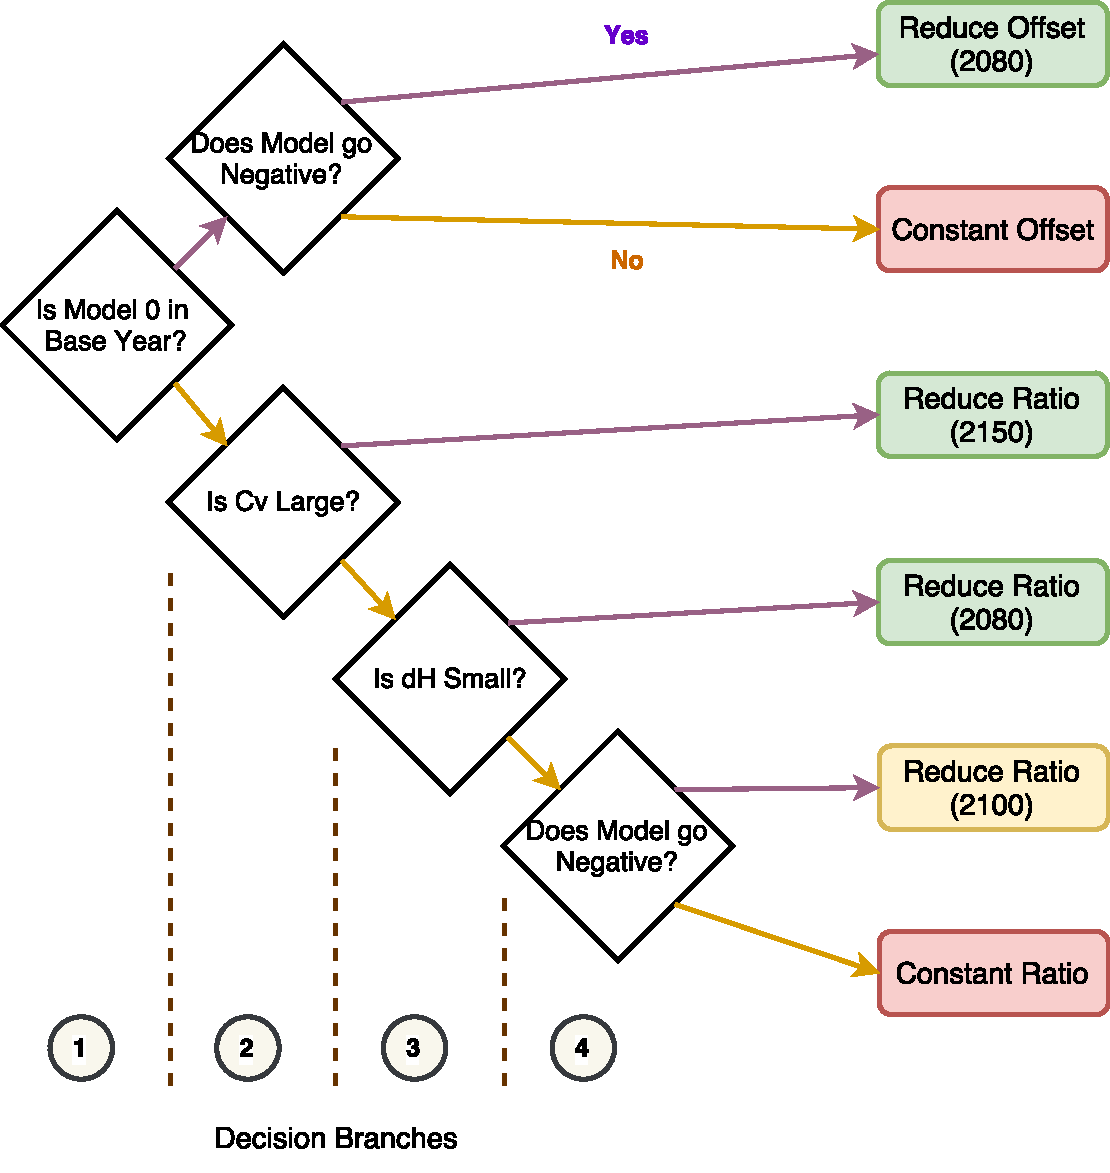
\includegraphics[width=\textwidth]{decision_tree.pdf}
    \caption[]{
      \label{fig:decision_tree}
      The default method decision tree used in the \code{aneris} software
      library. For all decisions, upper (purple) branches represent a ``yes''
      response and lower (orange) branches represent a ``no'' response. The
      coefficient of variation, $c_v$, is defined in Equation \ref{eqs:cov},
      $dH$ is defined as $\left|\frac{h(t_i) - m(t_i)}{h(t_i)}\right|$, and
      decision-making thresholds for $c_v$ and $dH$ are described below.  Where
      present, convergence years of default methods are provided below the
      method name in parentheses.  Methods labeled in \textit{green} are likely
      to closely match unharmonized results, methods in \textit{yellow} will
      likely somewhat match unharmonized results, and methods in \textit{red}
      can be expected to have a large relative difference between harmonized and
      unharmonized results.}
  \end{center}
\end{figure}

A number of characteristics impact the decision of which default method to
select based on the effect of the characteristic on the potential harmonized
trajectory. For example, it is possible for models to report zero values in the
harmonization year in situations in which technologies are introduced in future
time periods in regions or for sectors which produce an emissions species that
is absent in the initial modeling period. In such cases, an offset method is
required as a ratio method would mask future emissions and erroneously harmonize
the trajectory. 

In most cases, however, models do report values in the harmonization
year. Figure \ref{fig:cases} displays a number of illustrative example
trajectories which highlight the possible issues resulting from harmonizing
model results in different contexts. Panels \code{a} and \code{b} highlight
examples where model results peak mid-century, behavior that is seen in a number
of scenarios with general emissions mitigation effects, such as pollution
controls applied by developing nations on transport and industry sectors. Panel
\code{a} highlights a case where model base-year values and history are relative
close whereas Panel \code{b} shows a situation where model values and history
are relatively far apart. Panels \code{c} and \code{d} show similar model
trajectories that peak mid-century but also have negative emissions. Models can
report negative emissions in contexts in which a gas species which can be
extracted from the environment and stored, as is the case for \cotwo in future
scenarios with climate mitigation enacted via the deployment of carbon capture
and sequestration technologies or direct carbon capture technologies. Again, the
relative difference with historical values differ between the panels to explore
harmonization method choices in each situation.

When model and historical values are relatively close, a convergence method is
chosen in order to be as representative as possible to the underlying
unharmonized model results (Figure \ref{fig:cases}, Panel \code{a}). If values
are not close, the constant ratio method is chosen in order to provide
reasonable trajectories that still incorporate modeled effects (Figure
\ref{fig:cases}, Panel \code{b}).

If a model provides a trajectory that transitions from positive to negative
emissions and base year results are similar, then a convergence method is used
in order to guarantee capture of this transition in a representative fashion
(Figure \ref{fig:cases}, Panel \code{c}). If the discrepancy in base year
results is large, it is possible for a negative trajectory to be inappropriately
harmonized to a positive, but decreasing, trajectory. As such, the constant
ratio method is chosen (Figure \ref{fig:cases}, Panel \code{d}).

\begin{figure}
  \begin{center}
    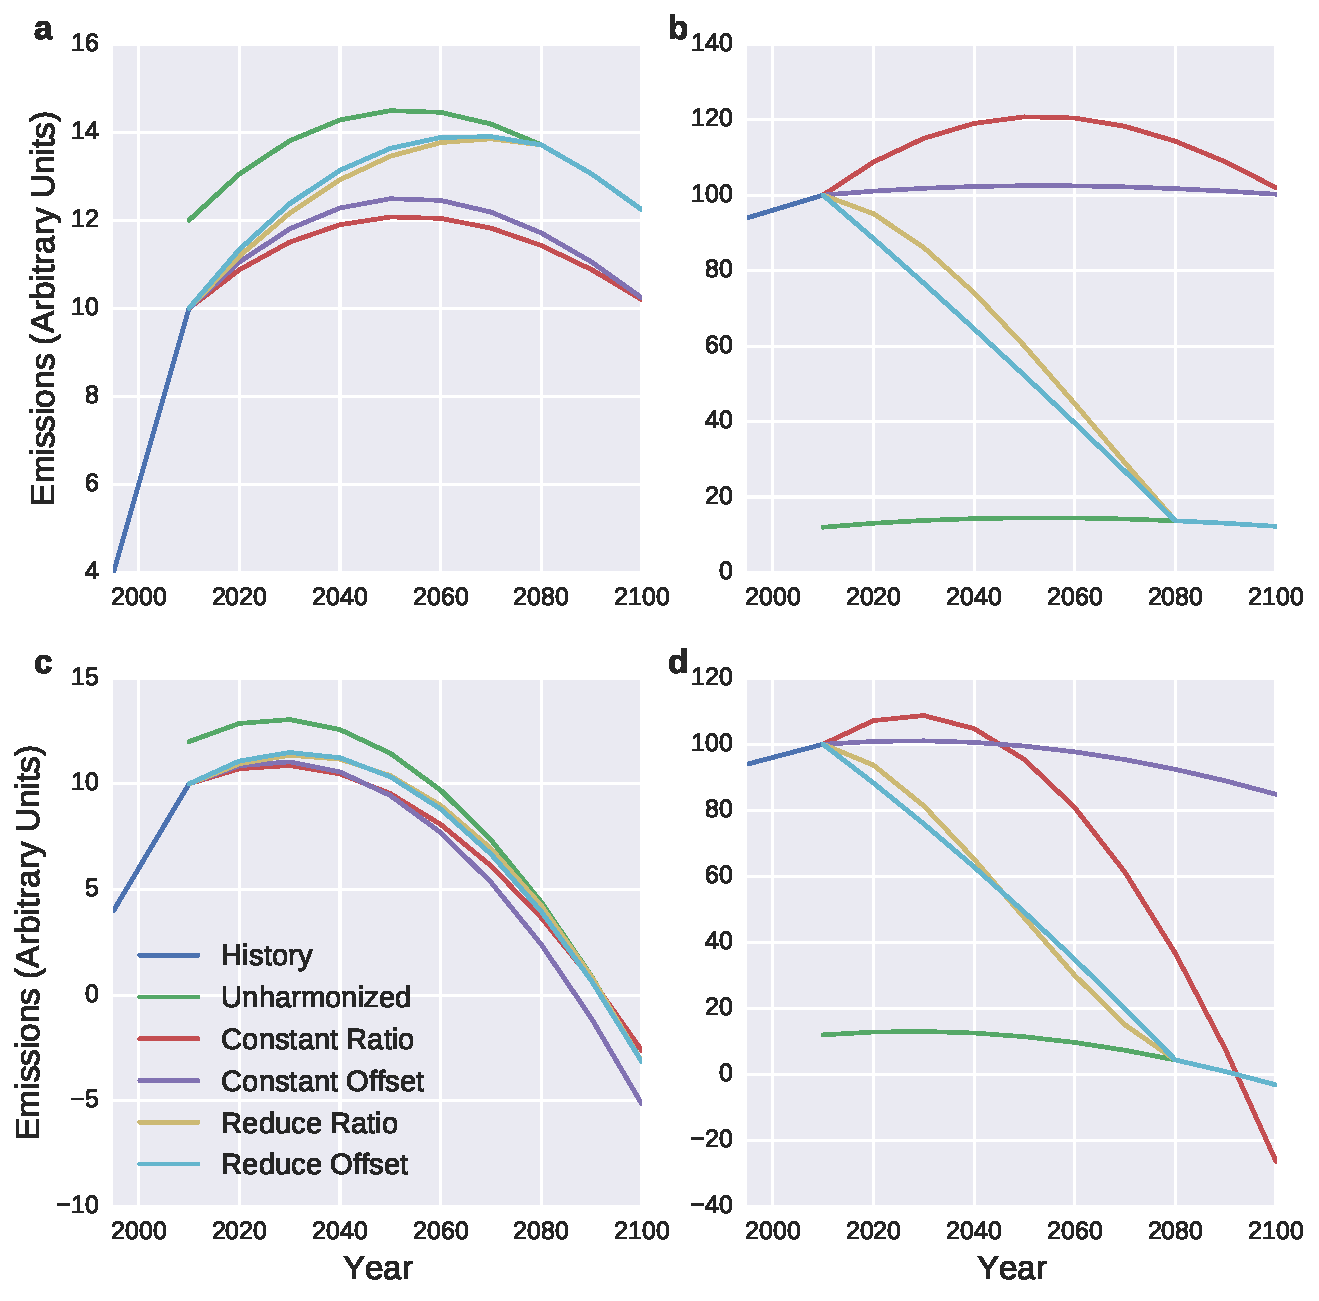
\includegraphics[width=\textwidth]{cases.pdf}
    \caption[]{
      \label{fig:cases}
      The effect of different harmonization routines on model trajectories under
      ``normal'' circumstances (Panel \code{a}), when there is a large
      difference between historical and model values in the harmonization year
      (Panels \code{b} and \code{d}), and when model trajectories result in
      negative emissions by the end of the modeling time horizon (Panels
      \code{c} and \code{d}). Identical model trajectories are used in each row
      (Panels \code{a}, \code{b}; \code{c}, \code{d}). In each column,
      historical values are increased in the base year by an order of magnitude
      (from 10 to 100). In each Panel, a subset of the potential routines
      provide a better harmonization quality than others as described in the
      text.
    }
  \end{center}
\end{figure}

Temporal variability of the historical trajectory is also an important
characteristic when considering the choice of harmonization method.  Emissions
from forest and grassland fires, for example, vary from year to year due to a
combination of meteorological conditions and anthropogenic drivers. Land use
emissions in many \glspl{iam} are modeled using average emission factors and do not
capture conditions in a specific year. A longer convergence horizon is thus
desired in order to incorporate highly variable historical data with modeled
results as is consistency in harmonization method because the effects are
modeled similarly across regions and species. In order to detect emissions with
a high amount of variation, a measure of the coefficient of variation, $c_v$, of
the first derivative of the historical trajectory is calculated using the
standard deviation, $\sigma$, and the mean, $\mu$, as shown in Equation
\ref{eqs:cov}. For a single realiziation of $c_v$, the first derivative
information of the entire historical time period is utilized.

\begin{equation}\label{eqs:cov}
    c_v =  \frac{\sigma(h^{\prime}(t))}{\mu(h^{\prime}(t))}
\end{equation}

The value of $c_v$ is then tested against a threshold, $\tau_{c_v}$. To
determine this threshold, an analysis of the recent \gls{ceds} and \gls{luc} historical data
has been performed. Figure \ref{fig:cov} shows the distribution of \gls{luc} $c_v$s
and non-\gls{luc} $c_v$s as determined for historical data aggregated to the model
regions of 5 different \glspl{iam} involved in the \gls{ssp} process: AIM-CGE, IMAGE, GCAM4,
MESSAGE-GLOBIOM, and REMIND-MAGPIE \TODO{add refs}, each of which have varying
definitions of native model regions comprising different collections of
countries. Therefore, each data point comprising Figure \ref{fig:cov} represents
a realization of $c_v$ for a single combination of native model region, sector,
and emissions species \footnote{A full listing of all sectors and species is
  presented in the case-study discussion in Section \ref{sec:results}, Table
  \ref{tab:sp}}. A threshold value of $\tau_{c_v} = 20$ has been chosen based on
these observations as it optimally divides the two distributions. Importantly,
tails of the \gls{luc} and non-\gls{luc} overlap, thus there are both false positives (~7\%
of non-\gls{luc} trajectories) and false negatives (~10\% of \gls{luc}
trajectories). However, as any regional definition is model dependent and thus
any regional aggregation is possible an automated detection mechanism is
necessary.


\begin{figure}
  \begin{center}
    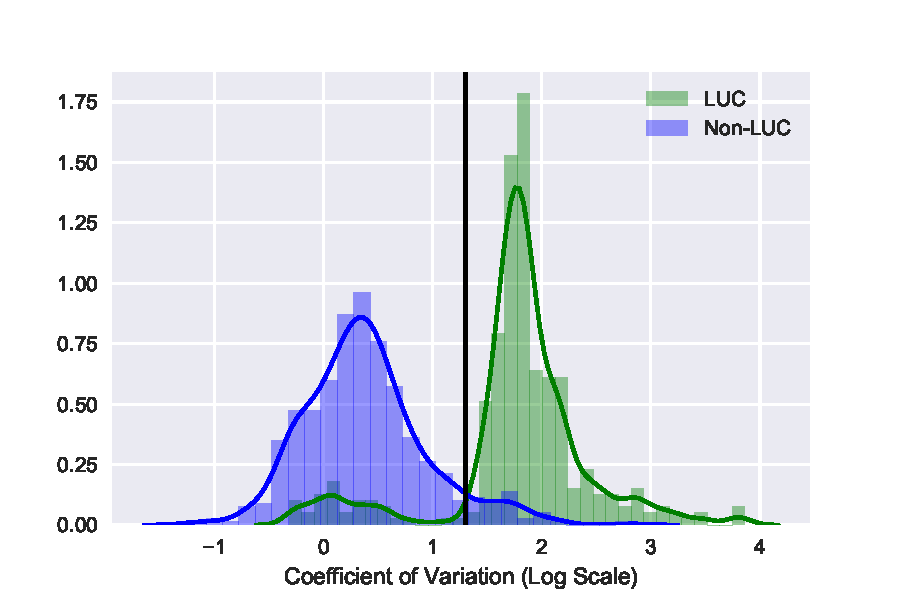
\includegraphics[width=\textwidth]{cov.pdf}
    \caption[]{
      \label{fig:cov}
      The distribution of $c_v$ values for \gls{luc} and non-\gls{luc} historical
      trajectories is shown. \gls{ceds} historical data \cite{hoesly_historical_2017}
      is used for non-\gls{luc} data and \cite{van_marle_historic_2017} is used for
      \gls{luc} data. All historical data has been aggregated from their native
      spatial resolution (i.e., individual countries) to \gls{iam} model regional
      definitions (i.e., collections of countries), and all gas species included
      in the historical data sets are included in the analysis. The solid black
      line indicates the threshold value, $\tau_{c_v}$, used by default in
      \code{aneris}.  }
  \end{center}
\end{figure}

Finally, consideration is taken with respect to the relative difference between
the historic and model values in the harmonization time period. In order to
investigate the possible values that these relative differences can take, the
\gls{iam} values used in the \gls{ssp} and (ongoing) \gls{cmip6} inter-comparison
exercises are used. A distribution of these differences for all models in the
study is presented in Figure \ref{fig:dh}. Given the available data, a threshold
value of $\tau_{dH} = 50$\% was chosen to be used as a default in \code{aneris}.

\begin{figure}
  \begin{center}
    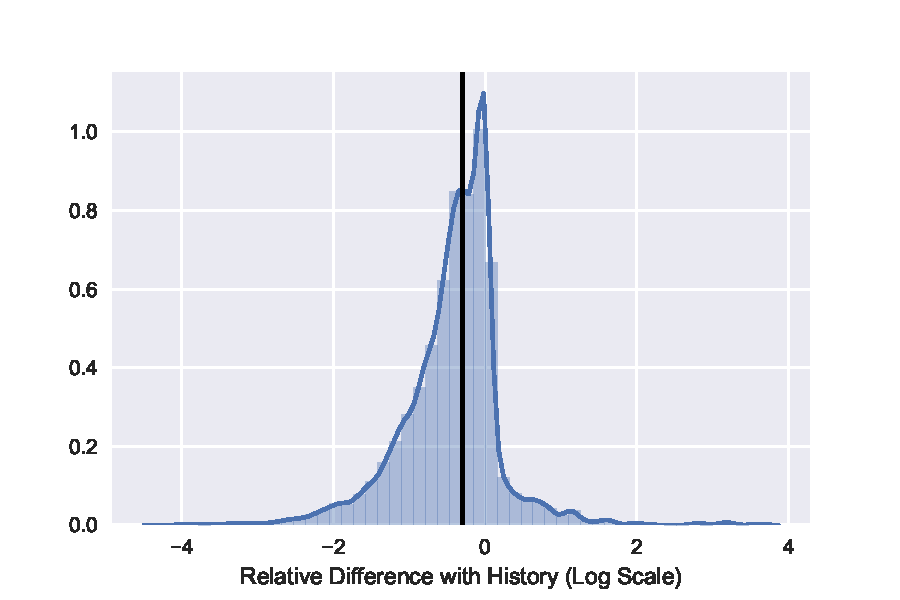
\includegraphics[width=\textwidth]{dh.pdf}
    \caption[]{
      \label{fig:dh}
      The distribution of relative differences between model and historical
      values in the harmonization year is shown. The solid black line indicates
      the 50\% threshold value, $\tau_{dH}$, used by default in \code{aneris}.
    }
  \end{center}
\end{figure}

\subsection{\code{aneris} Python Implementation and Workflow}\label{sec:workflow}

We herein present \code{aneris}' Python implementation, depicted in Figure
\ref{fig:software}, and conceptual, depicted in Figure \ref{fig:workflow}. The
library is composed of a number of utilities as well as three primary
components: the \texttt{HarmonizationDriver}, \texttt{Harmonizer}, and data
processing routines (shown in red, green, and blue, respectively in Figures
\ref{fig:software} and \ref{fig:workflow}).

The \texttt{HarmonizationDriver} is an object designed to interface with
user-provided data and configuration files. Input data (i.e., unharmonized model
results) is assumed to be an Excel file in the standard data format within the
\gls{iam} community, i.e., with \code{Model}, \code{Scenario}, \code{Region},
\code{Variable}, and \code{Unit} columns in addition to columns representing
each modeled time period. It is responsible for down-selecting data into
separate datasets for each model and scenario, invoking the harmonization
process on each dataset, and recompiling the results. The
\texttt{HarmonizationDriver} acts the primary interface for high-level users as
shown by the usage of the \texttt{driver} object in Listing
\ref{lst:tutorial}. Furthermore, a \gls{cli} is provided to allow users to more
easily incorporate the harmonization process in scripted workflows (Listing
\ref{lst:cli}, Figure \ref{fig:software}).

\begin{listing}[H]
\begin{minted}{python}
from aneris.tutorial import load_data
model, hist, driver = load_data()
for scenario in driver.scenarios():
    driver.harmonize(scenario)
harmonized, metadata = driver.harmonized_results()
\end{minted}
\caption{High-level user interaction with the \texttt{HarmonizationDriver} taken from the online \href{http://mattgidden.com/aneris/config.html}{tutorial}}
\label{lst:tutorial}
\end{listing}

\begin{listing}[H]
\begin{minted}{bash}
$ aneris -h
usage: aneris [-h] [--history HISTORY] [--regions REGIONS] [--rc RC]
              [--output_path OUTPUT_PATH] [--output_prefix OUTPUT_PREFIX]
              input_file

    Harmonize historical trajectories to data in the IAM template format.

    Example usage:

    aneris input.xlsx --history history.csv --regions regions.csv

positional arguments:
  input_file            Input data file.

optional arguments:
  -h, --help            show this help message and exit
  --history HISTORY     Historical emissions in the base year.
  --regions REGIONS     Mapping of country iso-codes to native regions.
  --rc RC               Runcontrol YAML file (see
                        http://mattgidden.com/aneris/config.html for
                        examples).
  --output_path OUTPUT_PATH
                        Path to use for output file names.
  --output_prefix OUTPUT_PREFIX
                        Prefix to use for output file names.
\end{minted}
\caption{The \gls{cli} help provided by the \code{aneris} package.}
\label{lst:cli}
\end{listing}

The \texttt{Harmonizer} is a Python class whose concern is to harmonize model
value trajectories given historical data and possible user method
\textit{overrides}, i.e., non-default methods (described further below). It is
used by the \texttt{HarmonizationDriver}; however it is also available to the
user as a first-class object. The \texttt{Harmonizer} requires that input data
conform to the \code{aneris} calculation data format, which explicitly separates
the emissions species from the sector contributing the emissions (these are
combined in the single \code{Variable} column in the standard \gls{iam}
format). Because the \texttt{Harmonizer} is designed to operate on a single
instance of a model and scenario, the canonical data format includes
\texttt{region}, \texttt{sector}, \texttt{gas}, and \texttt{units} columns
without extraneous metadata columns for the model and scenario. Once configured
with appropriate input data (model and history) as well as potential method
overrides, the \texttt{Harmonizer}'s \texttt{harmonize()} method can be invoked
which returns a \texttt{pandas.DataFrame} of harmonized data. The object can
additionally be queried directly as to its \texttt{default\_methods()},
\texttt{methods()} (i.e., methods used with overrides), and \texttt{metadata()}
(i.e., methods used with all branching information along each path in the
decision tree).

There are also a variety of tools and utilities provided to users and also used
by the \texttt{HarmonizationDriver} in order to process both input and output
data. These include an \texttt{EmissionsAggregator} class and related routines
used to generate sectoral emissions totals, generate regional totals, and
combine historical emissions to native model regions (where historical data is
defined at a higher spatial resolution than a model; see, e.g., Figure
\ref{fig:regions}). A \texttt{FormatTranslator} class is also provided which
defines an interface for translating \texttt{pandas.DataFrame}s between the \gls{iam}
format expected for input and output data and the calculation format used by
\code{aneris}' \texttt{Harmonizer}.

\begin{figure}
  \begin{center}
    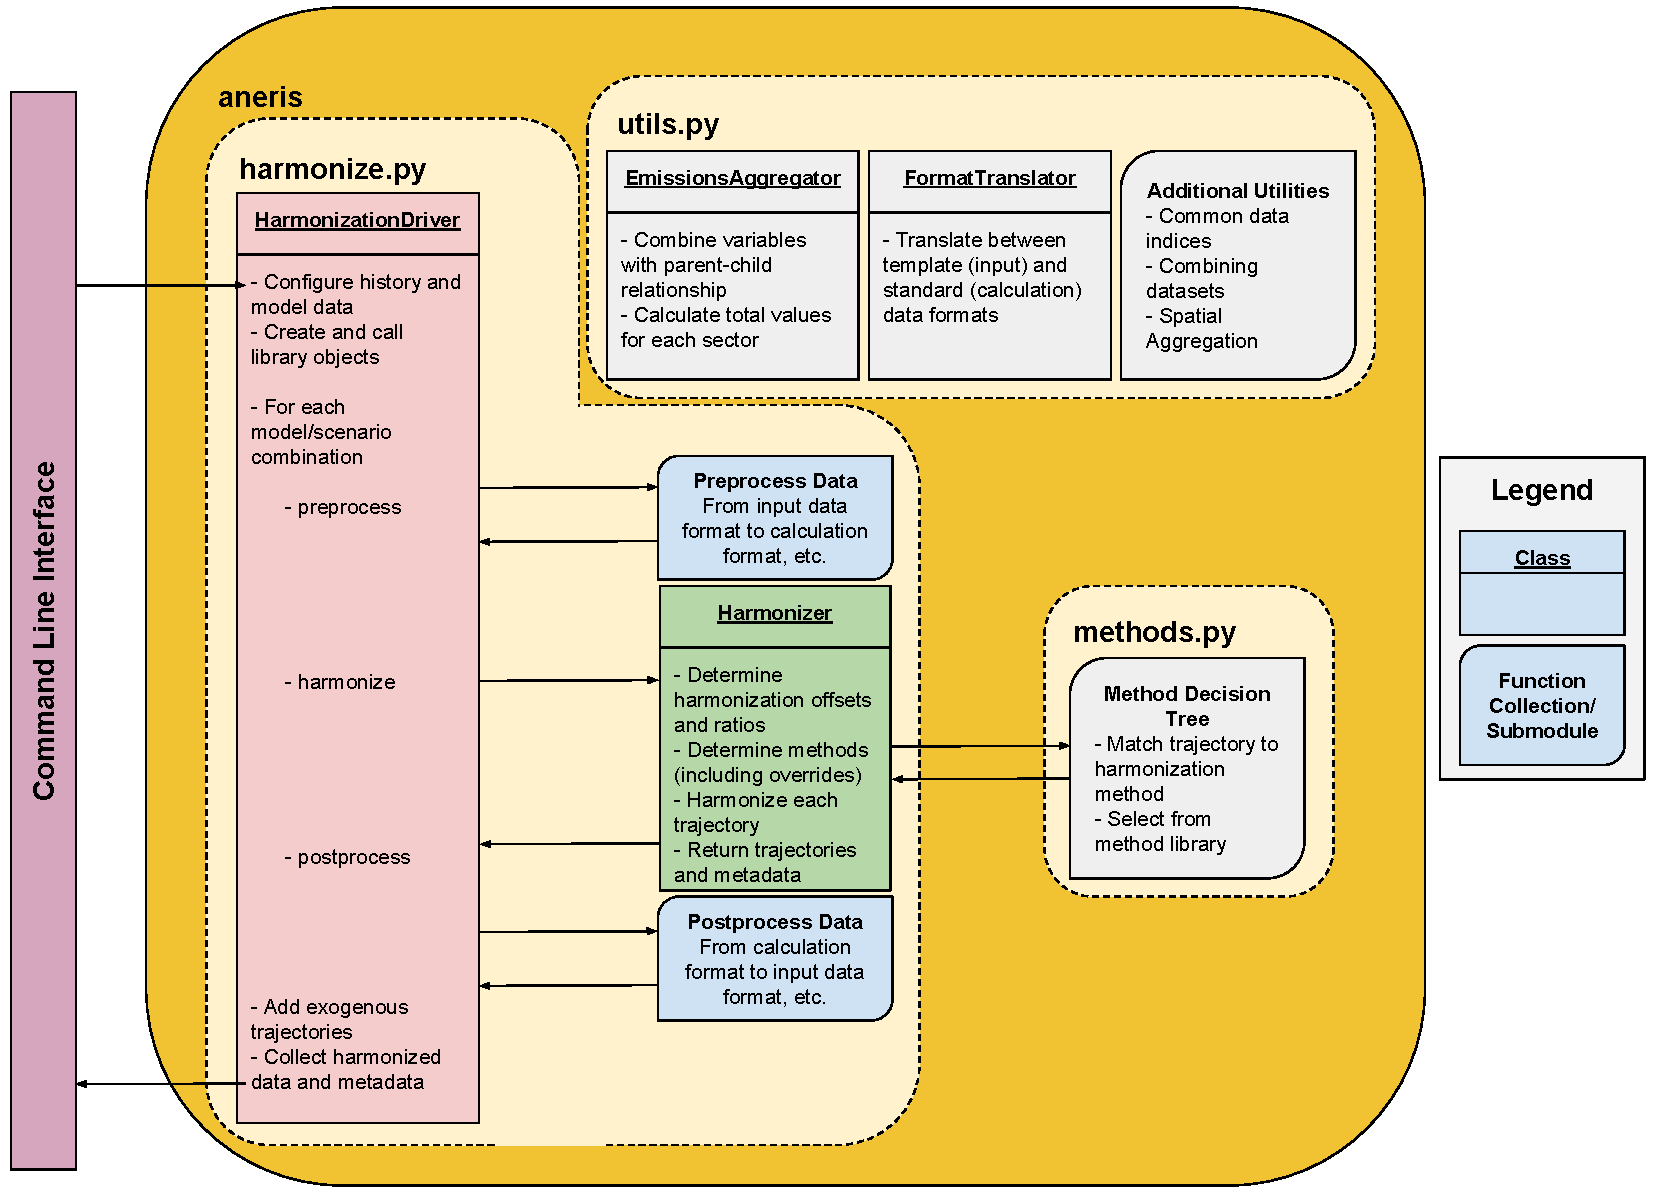
\includegraphics[width=\textwidth]{implementation_schematic.pdf}
    \caption[]{
      \label{fig:software}
      The various objects and their relation to one another in the \code{aneris}
      code base as well as a short description of their scope of concern.  
    }
  \end{center}
\end{figure}

\begin{figure}
  \begin{center}
    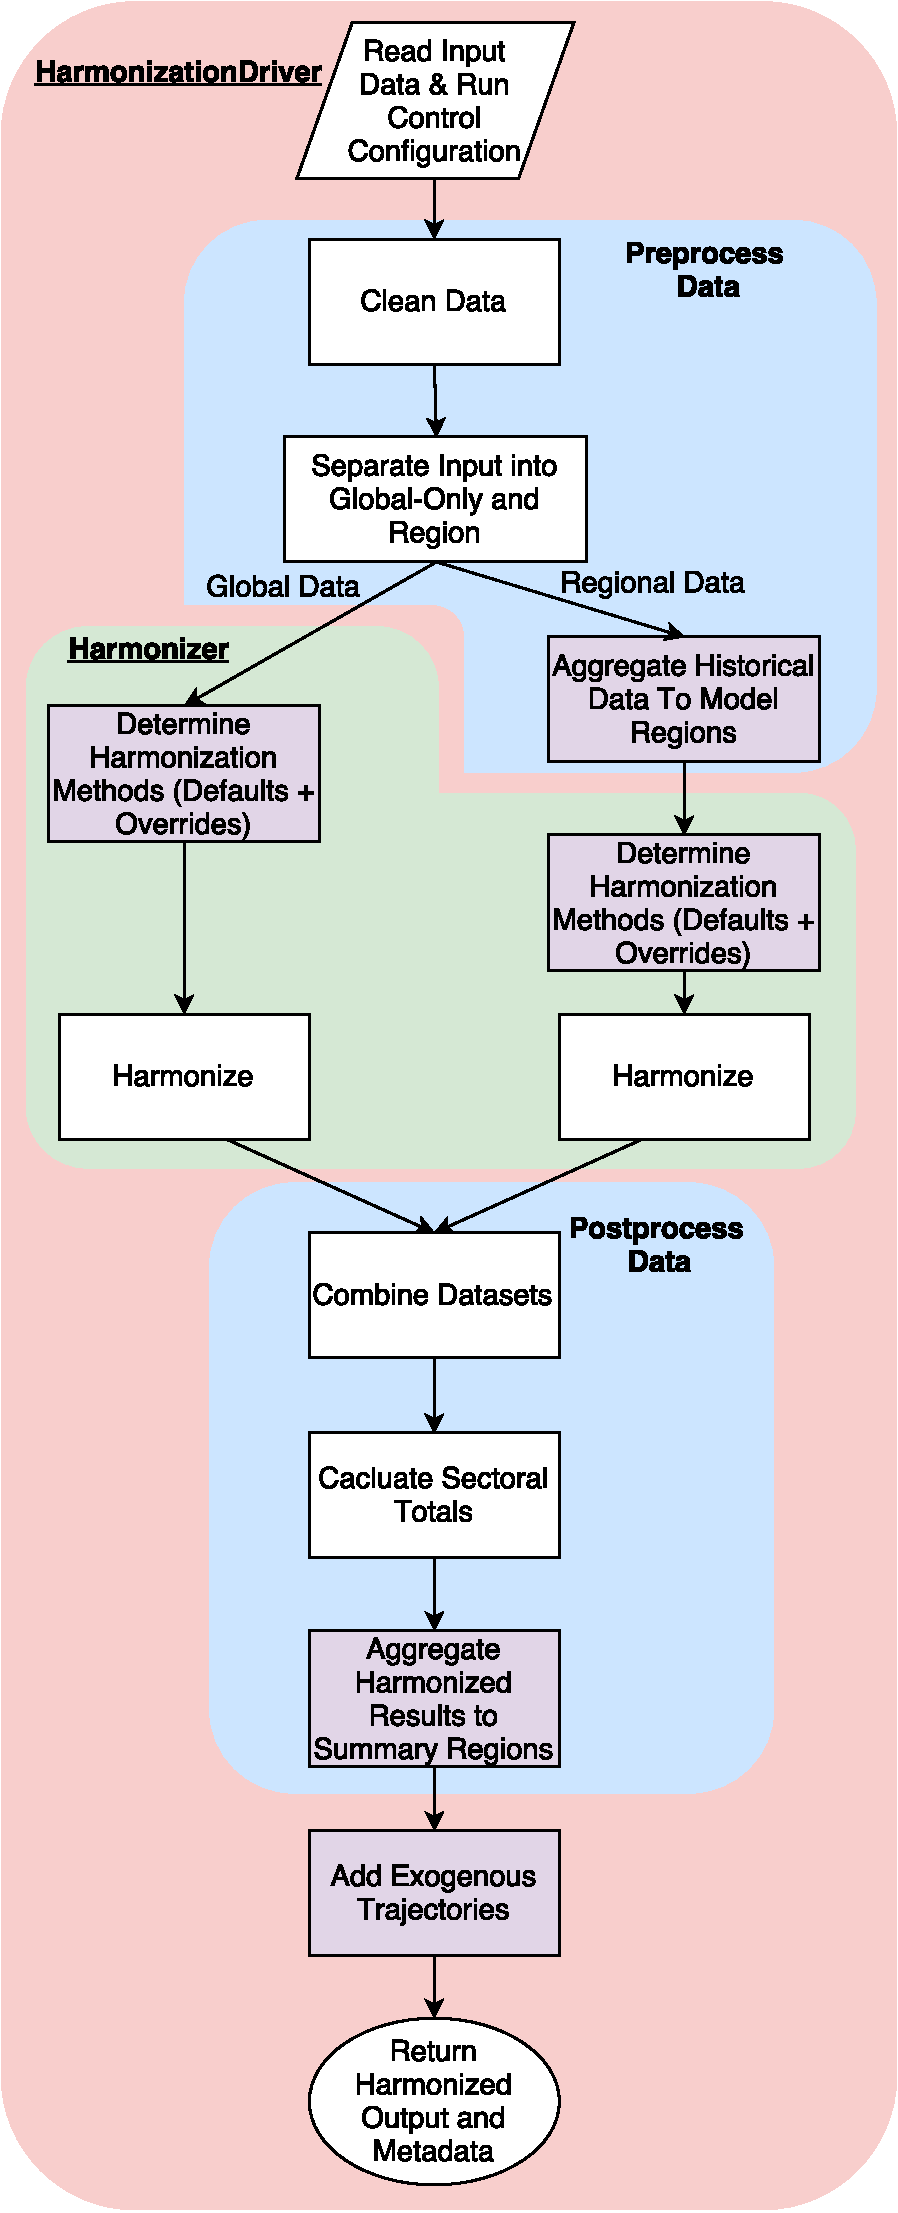
\includegraphics[height=0.8\textheight]{aneris-workflow.pdf}
    \caption[]{
      \label{fig:workflow}
The full harmonization process as executed by \code{aneris} for a single
instance of a model and scenario. Operations that can be configured with
user-based input configurations are shown in purple. Operations governed by the
\texttt{HarmonizationDriver} are shown in red. Data processing operations are
shown in blue. The core harmonization process, governed by the
\texttt{Harmonizer} is shown in green. }
  \end{center}
\end{figure}

%% \begin{figure}
%%   \subfloat[Python Implementation\label{fig:software}]{
%%     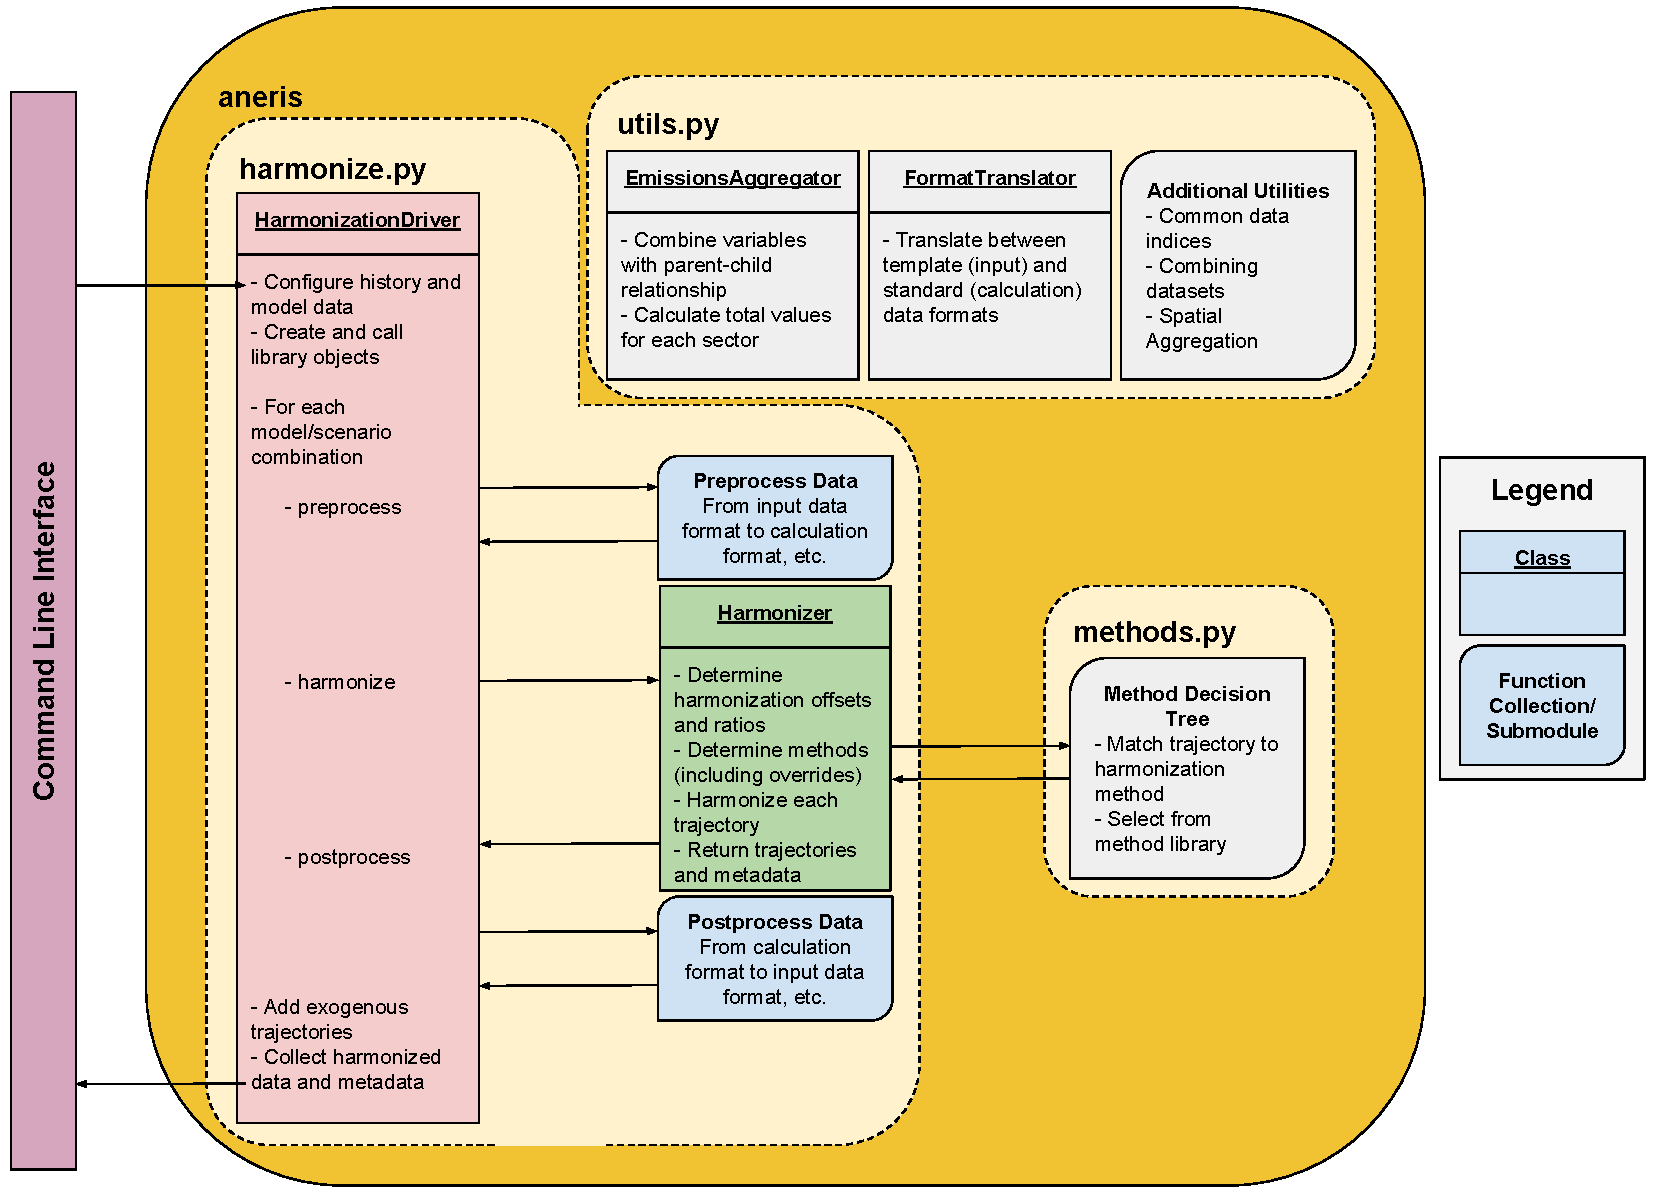
\includegraphics[width=0.775\textwidth]{implementation_schematic.pdf}
%%     }
%%   \subfloat[Workflow\label{fig:workflow}]{
%%     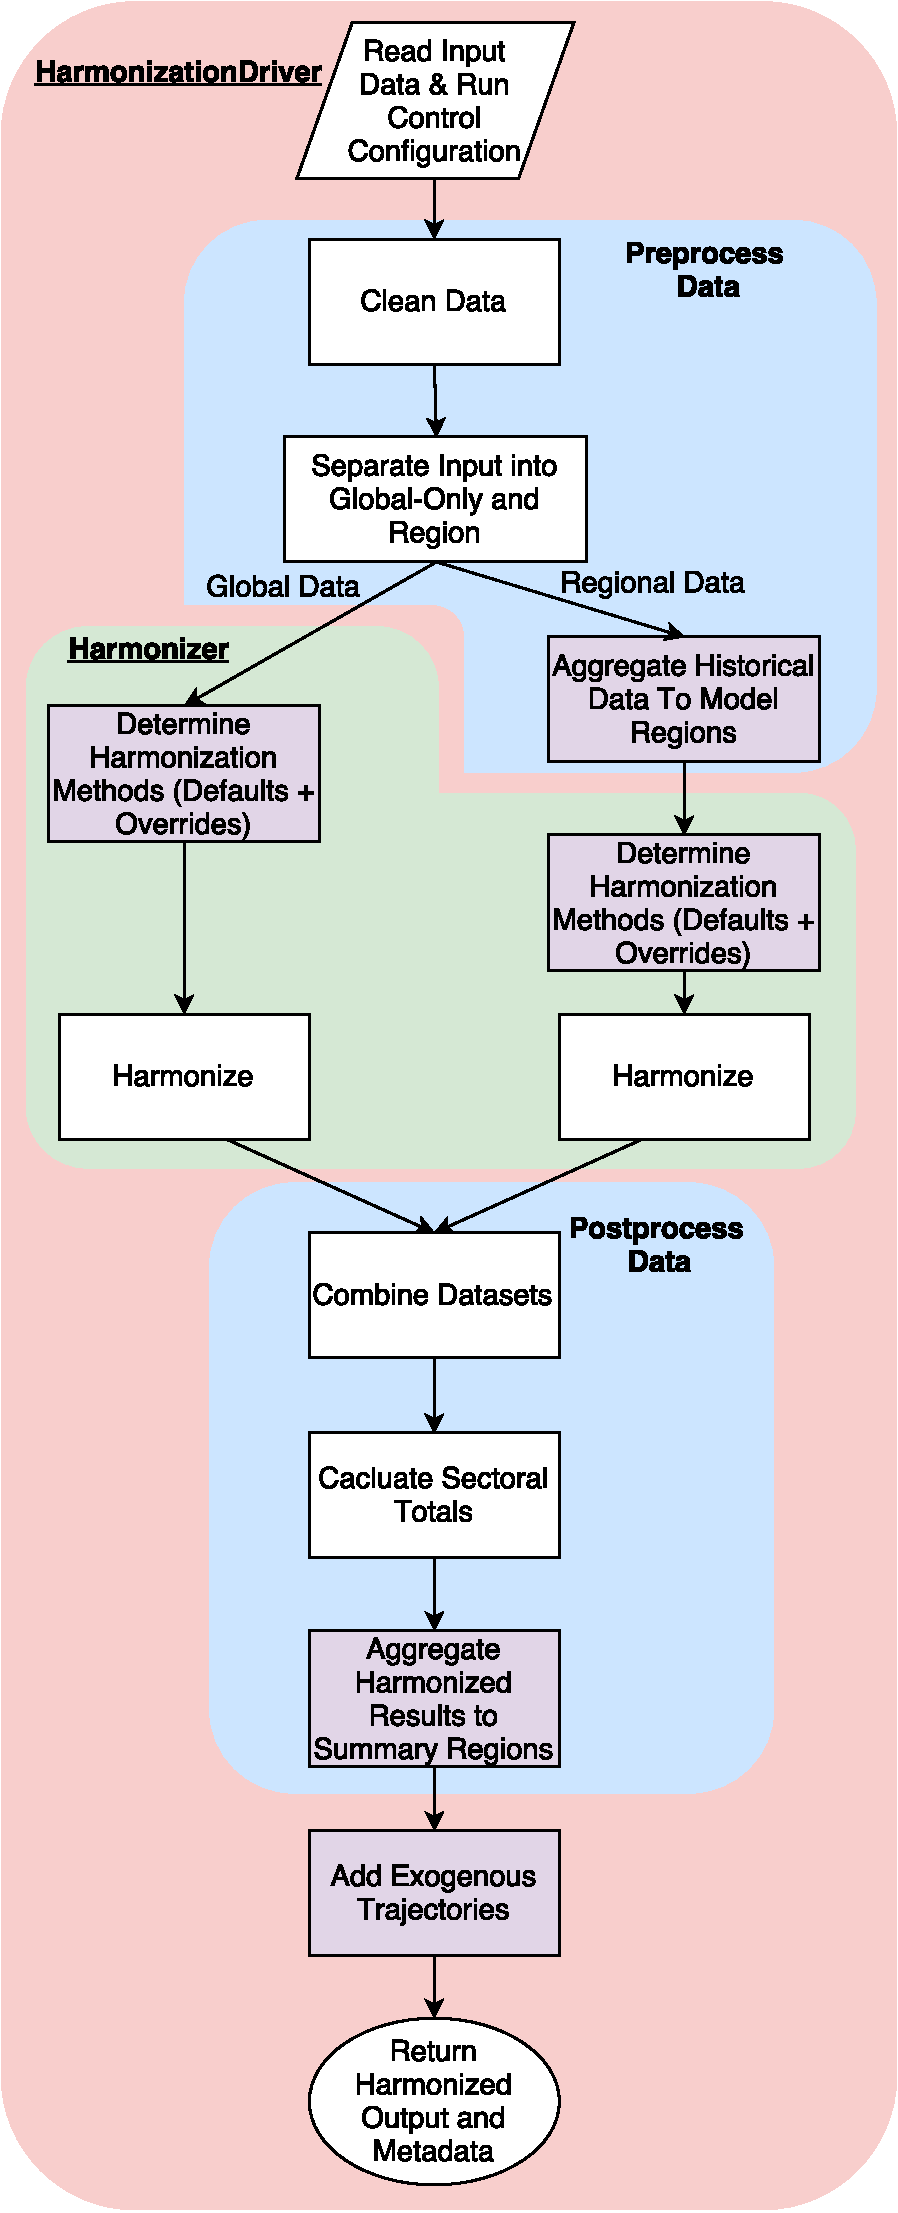
\includegraphics[width=0.225\textwidth]{aneris-workflow.pdf}
%%     }
%%     \caption{ Panel \ref{fig:software} shows the various objects in the
%%       \code{aneris} code base as well as a short description of their scope of
%%       concern. Panel \ref{fig:workflow} displays the full harmonization process
%%       as executed by \code{aneris} for a single instance of a model and
%%       scenario. Operations that can be configured with user-based input
%%       configurations are shown in purple. Operations governed by the
%%       \texttt{HarmonizationDriver} are shown in red. Data processing operations
%%       are shown in blue. The core harmonization process, governed by the
%%       \texttt{Harmonizer} is shown in green.  }
%%     \label{fig:software-workflow}
%% \end{figure}

The full harmonization workflow, outlined in Figure \ref{fig:workflow}, begins
by cleaning input data, which adds (0-valued) model trajectories that exist in
the historical data set but are not provided by the model input and detects any
issues that would cause the harmonization process to fail. The methods used to
harmonize the data are then determined and the harmonization process is
executed. Upon completion of the harmonization process, aggregation of common
analysis regions is performed. A common regional aggregation used in the
\gls{iam} community was defined in the \glspl{rcp}
\cite{vuuren_representative_2011}, shown in Figure \ref{fig:regions}. Finally,
any exogenous trajectories the user provides are added. Exogenous trajectories
are normally provided for unmodeled gases with well-accepted scenario
trajectories, e.g., chlorofluorocarbons provided by the \gls{wmo}
\cite{wmo2014}. Upon completion, the harmonized trajectories and meta data
regarding the harmonization process are returned. A description of all returned
meta data is provided in Table \ref{tab:metadata}.

\begin{figure}
  \begin{center}
    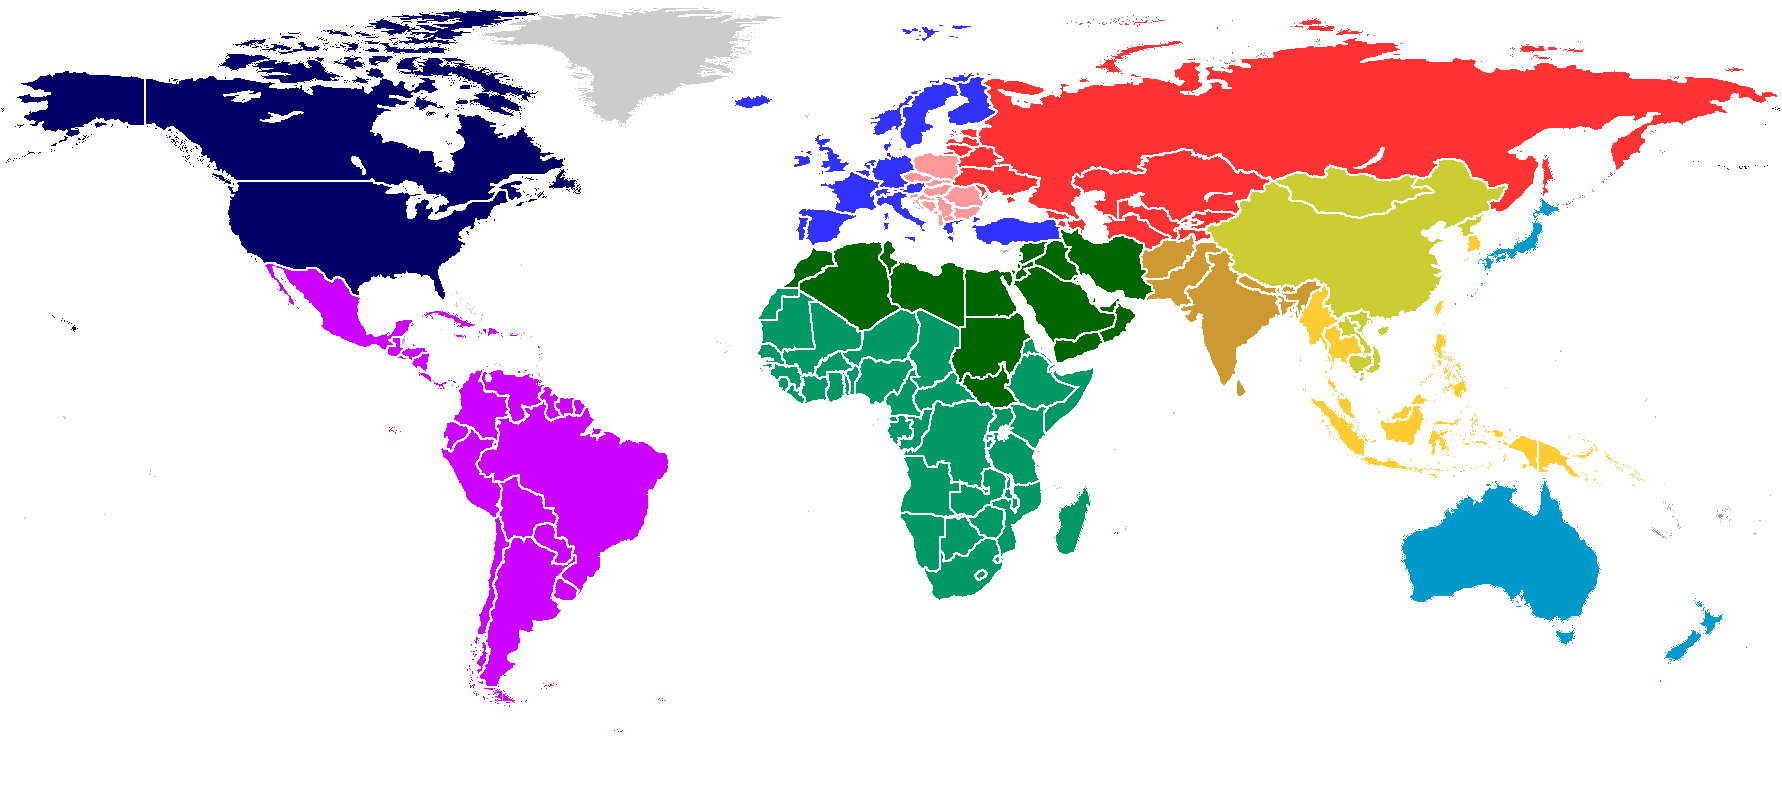
\includegraphics[width=\textwidth]{MESSAGE_11-5regions_map.pdf}
    \caption[]{
      \label{fig:regions}
      The 5 regions used in the \glspl{rcp} with their 11-region constituents: Asia
      (\gls{cpa}, \gls{sas}, \gls{pas}) [yellows], \gls{lam}
      [magenta], the \gls{mea} and \gls{afr} [greens], the OECD (\gls{nam},
      \gls{weu}, and \gls{pao}) [blues], and the Reforming Economies
      (\gls{eeu} and \gls{fsu}) [reds].  }
  \end{center}
\end{figure}

\begin{table}[]
\centering
\caption{Meta data provided by the \code{aneris} harmonization routine. This meta data is provided for every combination of region, sector, and emissions species.}
\label{tab:metadata}
\begin{tabular}{|p{2cm}|p{8cm}|}
\hline
\textbf{Column}       & \textbf{Description}                                      \\
\hline
\hline
method       & The harmonization method used.                                               \\
\hline
default      & The default harmonization method as determined by the default decision tree. \\
\hline
override     & The method provided as an override (if any).                                 \\
\hline
offset       & The offset value between history and model in the harmonization year.        \\
\hline
ratio        & The ratio value between history and model in the harmonization year.         \\
\hline
cov          & The coefficient of variation value of the historical trajectory.                           \\
\hline
unharmonized & The unharmonized value in the harmonization year.                            \\
\hline
history      & The historical value in the harmonization year.                             \\
\hline
harmonized   & The resulting harmonized value in the harmonization year.\\
\hline
\end{tabular}
\end{table}

Users are able to control the harmonization process via a number of options
(with examples provided
\href{http://mattgidden.com/aneris/config.html}{online}). The primary mechanism
by which users control the process is by providing \textit{override} methods for
any combination of region and variable (i.e., sector and gas species).  In
practice, it may be possible that not all default methods chosen will provide
robust harmonized trajectories, especially if there is a significant difference
between historical and model values in the harmonization year, if there is
significant upward or downward movement in the model trajectory, or if there are
known discrepancies in sectoral definition between the \gls{iam} and historical data
source. In such cases, users can override default methods with their method of
choice and both the default method and override is reported in the resulting
metadata.

In order to help identify cases where overrides may be of interest,
harmonization \textit{diagnostics} are provided which analyze the relative
difference between harmonized and unharmonized trajectories at their mid and
end-points. These values are configurable by the user, but defaults of $400$\%
and $200$\%, respectively, are provided based on experiences of the authors'
using \code{aneris} to date.

\section{Case Study: Harmonizing Results from a Global IAM}\label{sec:results}

In order to show a representative cross section of the performance of the
\code{aneris} harmonization procedure, we focus on the harmonization of results
of the \gls{iam} MESSAGE-GLOBIOM \cite{fricko_marker_2017}. Two scenarios from the \gls{ssp}
scenario library \cite{Riahi2017153,Rao2017346} are presented. The SSP2, or
``middle of the road'', scenario (referred to as SSP2-Ref) is chosen to be
analyzed because MESSAGE-GLOBIOM is the marker scenario for this \gls{ssp}. This SSP2
scenario lies between two \glspl{rcp}, 6 and 8.5, with a radiative forcing level of
approximately 6.5 Wm$^{-2}$. We additionally present the results for the
SSP2-based mitigation scenario leading to a radiative forcing of 4.5 Wm$^{-2}$
(referred to as SSP2-4.5). The SSP2-45 scenario is chosen because mitigation
technologies and policies are enacted causing a general reduction in pollutants
and \glspl{ghg}, including (eventual) negative \cotwo emissions in some regions and
sectors due to carbon capture and sequestration and afforestation. A scenario in
which negative emissions play a role in mitigation strategies is particularly
important because of the sensitivity of key indicators, such as end-of-century
radiative forcing (which is used to estimate mean global temperature increase),
to the timing and magnitude of net-zero and total negative \cotwo
emissions. Therefore, these two scenarios represent two relative extreme cases
in the use of a harmonization approach and thus provide a case study as to its
general applicability. Figure \ref{fig:kyoto} shows the different trends of
Kyoto Gases in each scenarios.


\begin{figure}
  \begin{center}
    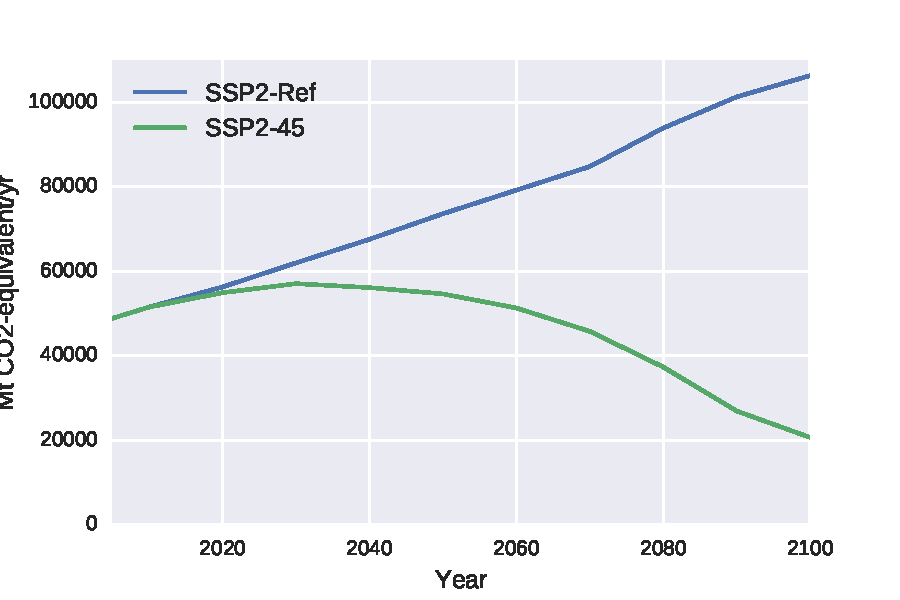
\includegraphics[width=\textwidth]{results_kyoto.pdf}
    \caption[]{
      \label{fig:kyoto}
      Unharmonized Kyoto gas emissions for SSP2-Ref, a scenario with generally
      increasing global emissions trends, and SSP2-45, a scenario with generally
      decreasing global emissions trends.  }
  \end{center}
\end{figure}


MESSAGE-GLOBIOM includes a representation of 11 distinct regions which can be
mapped directly to the 5-region definition used in the \glspl{rcp}. Historical data is
taken from previously described \gls{luc} and anthropogenic sources, which comprise 10
separate pollutant and \gls{ghg} species and 12 sectors shown in Table \ref{tab:sp}. A
total of 970 distinct trajectories were harmonized for each scenario, and
therefore 1940 trajectories were harmonized in total. \noxx generated from the
Energy sector provides an example of an emissions species and sector in which
all regions were satisfactorily harmonized with the default methods. Figure
\ref{fig:nox} shows the results of harmonization in Asia, and Table
\ref{tab:nox} describes the parameters that underlie the choice of method for
each harmonized trajectory.

\begin{table}[]\begin{minipage}{\textwidth}
  \centering
  \caption{Harmonized Species and Sectors}
  \label{tab:sp}
  \begin{tabular}{|l|l|}
    \hline
    \textbf{Emissions Species}        & \textbf{Sectors}                    \\
    \hline
    \hline
    Black Carbon (BC)                 & Agricultural Waste Burning          \\
    Hexafluoroethane (C\textsubscript{2}F\textsubscript{6})
    \footnote{\label{x_glb_all}
      Global total trajectories are harmonized due to lack of detailed 
      historical data.}
                                      & Agriculture                         \\
    Tetrafluoromethane (CF\textsubscript{4})
    \footnoteref{x_glb_all}               & Aircraft
    \footnote{\label{x_glb}
      Global sectoral trajectories are harmonized due to lack of detailed 
      historical data.}                            \\
    Methane (CH\textsubscript{4})                     & Energy Sector                       \\
    Carbon Dioxide (CO\textsubscript{2})
    \footnote{\label{x_co2}
      A global trajectory for land-use CO\textsubscript{2} is used; non-land-use sectors 
      are harmonized for each model region.}
                                      & Forest Burning                      \\
    Carbon Monoxide (CO)              & Grassland Burning                   \\
    Hydrofluorocarbons (HFCs)
    \footnoteref{x_glb_all}               & Industrial Sector                   \\
    Nitrous Oxide (N\textsubscript{2}O)
    \footnoteref{x_glb_all}
                                      & International Shipping\footnoteref{x_glb}              \\
    Ammonia (\nht)                     & Residential Commercial Other        \\
    Nitrogen Oxides (\nox)             & Solvents Production and Application \\
    Organic Carbon (OC)               & Transportation Sector               \\
    Sulfur Hexafluoride (SF\textsubscript{6})
    \footnoteref{x_glb_all}               & Waste                               \\
    Sulfur Oxides (SO\textsubscript{x})               &                                     \\
    Volatile Organic Compounds (VOCs) &                                     \\
    \hline
  \end{tabular}
\end{minipage}\end{table}


\begin{figure}
  \begin{center}
    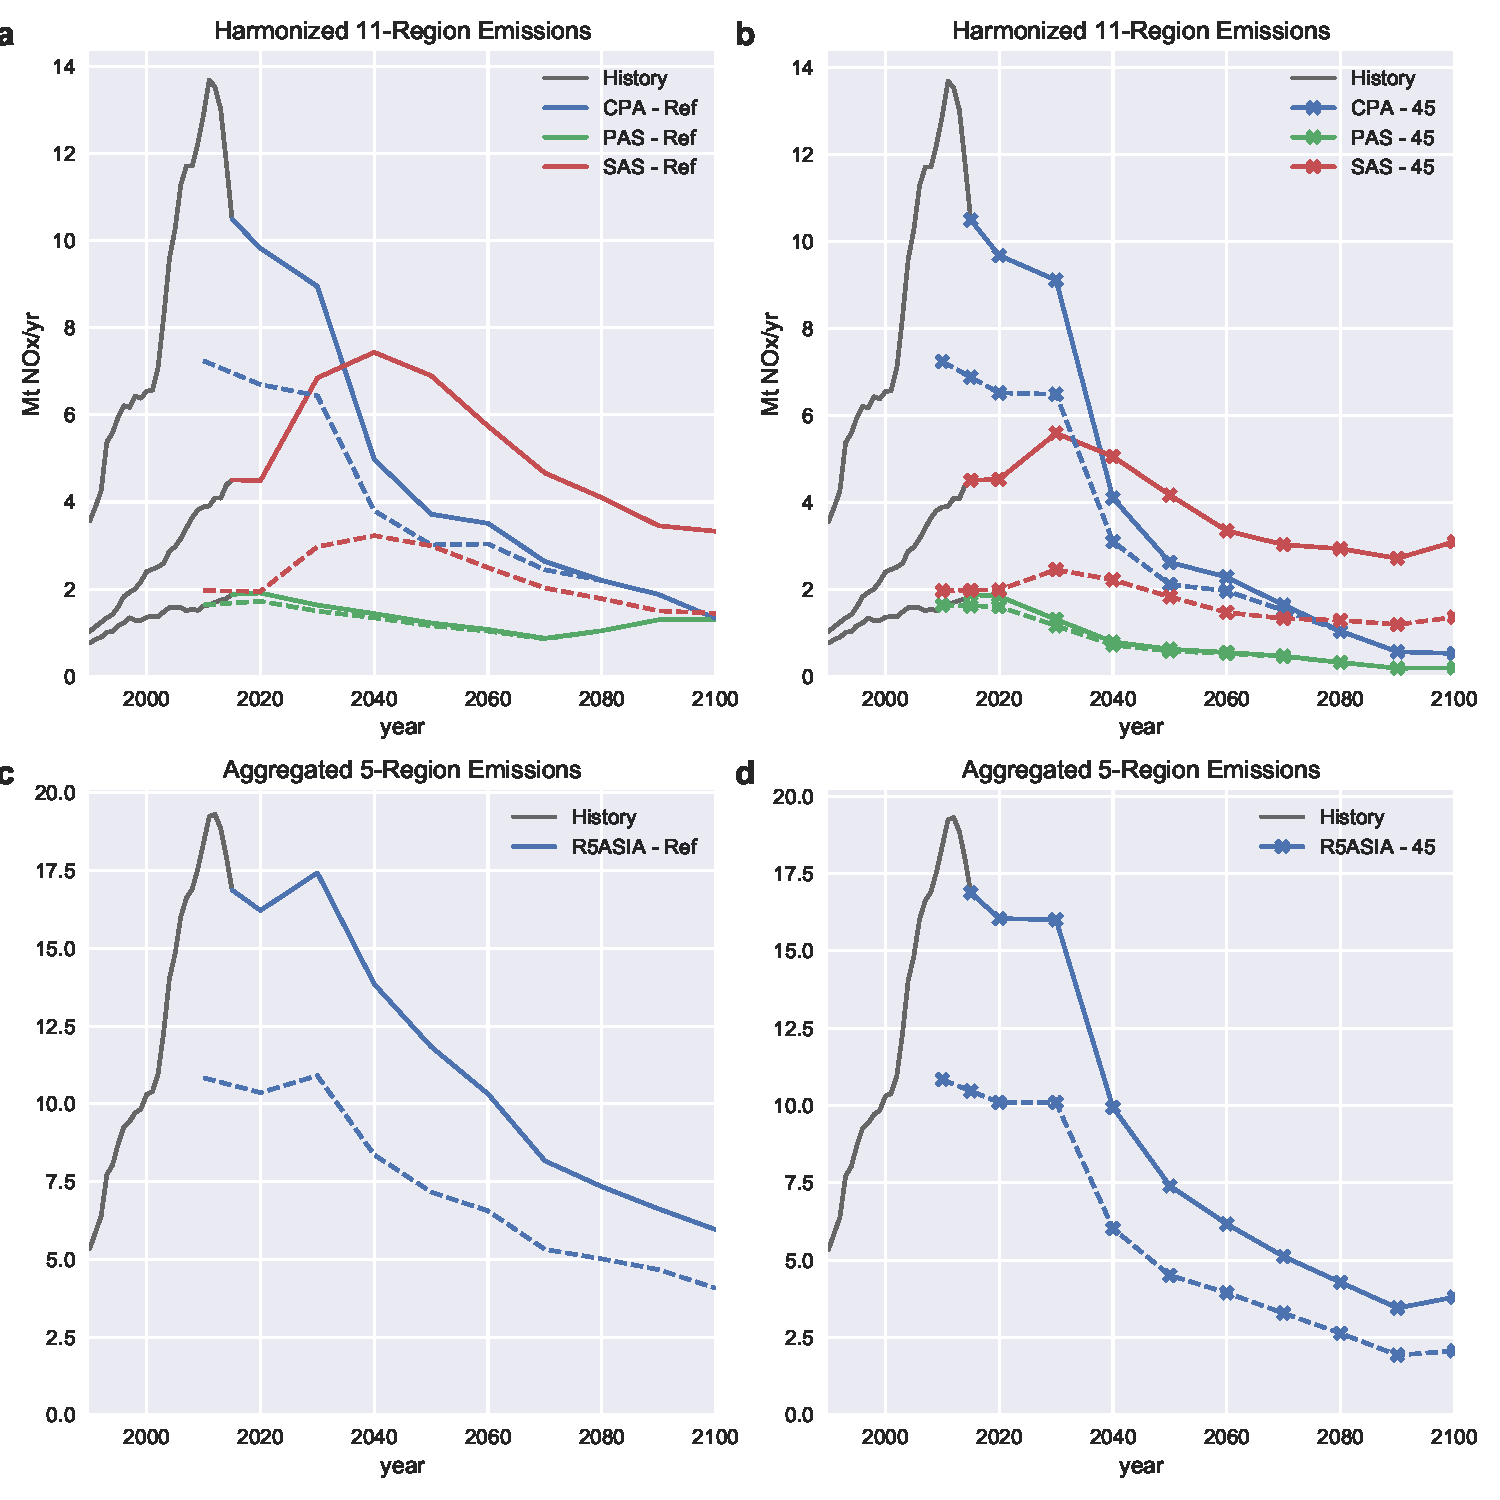
\includegraphics[width=\textwidth]{example_NOx_Energy_Sector.pdf}
    \caption[]{
      \label{fig:nox}
      \noxx Energy Sector harmonized (solid lines) and unharmonized (dashed lines)
      trajectories for SSP2 and SSP2-45 with historical trajectories (grey
      lines) are presented. The SSP2 reference scenario is shown in Panels
      \textbf{a} and \textbf{c}; the SSP-45 scenario is denoted with ``x''
      markers in Panels \textbf{b} and \textbf{d}. The upper panels show the
      results for endogenously modeled and harmonized regions in Asia while the
      lower panels display the aggregate region results.  
    }
  \end{center}
\end{figure}

\begin{table}[]
\centering
\caption{Key Parameters for Deciding Harmonization Methods for \noxx Emissions in the Energy Sector in Asia}
\label{tab:nox}
\begin{tabular}{|p{1.2cm}|p{.5cm}|p{.5cm}|p{4.5cm}|p{3cm}|}
\hline
\textbf{Region} & \textbf{dH} & $\mathbf{c_v}$ & \textbf{Decision Tree Traversal (Branch and Direction)} & \textbf{Default Method Chosen} \\ \hline
    \hline
CPA             & 0.35        & 2.26          & 1 (no), 2 (no), 3 (yes)                                 & reduce\_ratio\_2080    \\ \hline
PAS             & 0.14        & 1.24          & 1 (no), 2 (no), 3 (yes)                                 & reduce\_ratio\_2080    \\ \hline
SAS             & 0.56        & 0.58          & 1 (no), 2 (no), 3 (no), 4 (no)                          & constant\_ratio        \\ \hline
\end{tabular}
\end{table}

The harmonization of emissions pathways is performed in order to accurately
represent new or updated data sets of historical emissions inventories while also
maintaining consistency with the original, unharmonized pathway. As such, when
the default methods as provided by the harmonization procedure distort or
otherwise sufficiently misrepresent the underlying unharmonized results, an
override method is required to be provided for the trajectory of the region,
sector, and species in question. Of the 970 trajectories, approximately 10\%
were reported as a diagnostic (see Section \ref{sec:workflow}) of which 3.5\%
required the use of harmonization overrides after an initial investigation;
thus, 96.5\% of all trajectories were satisfactorily harmonized using the
default methods. The trajectories that required overrides clustered into two
classifications: regional trajectories whose \textit{magnitude} was overly
distorted and regional trajectories whose \textit{shape} was overly distorted.

Figure \ref{fig:co} presents a case in which the magnitude of a trajectory is
distorted. A large discrepancy ($\sim$300\% relative difference) is observed in
the harmonization year for carbon monoxide (CO) emissions in the industrial
sector specifically for the South Asia (SAS) MESSAGE-GLOBIOM region, which
comprises most of the emissions of the Asian subcontinent. The default method
chosen (\code{constant_ratio}) maintains model trends for the region; however,
overall model results are distorted. By applying a \code{constant_offset}
override, the regional trend and magnitude is maintained. With the new
harmonization method for the SAS region, the global trajectory for industrial CO
also is representative of the trends seen in the unharmonized trajectory and the
relative importance of the underlying regional trajectories is maintained.

\begin{figure}
  \begin{center}
    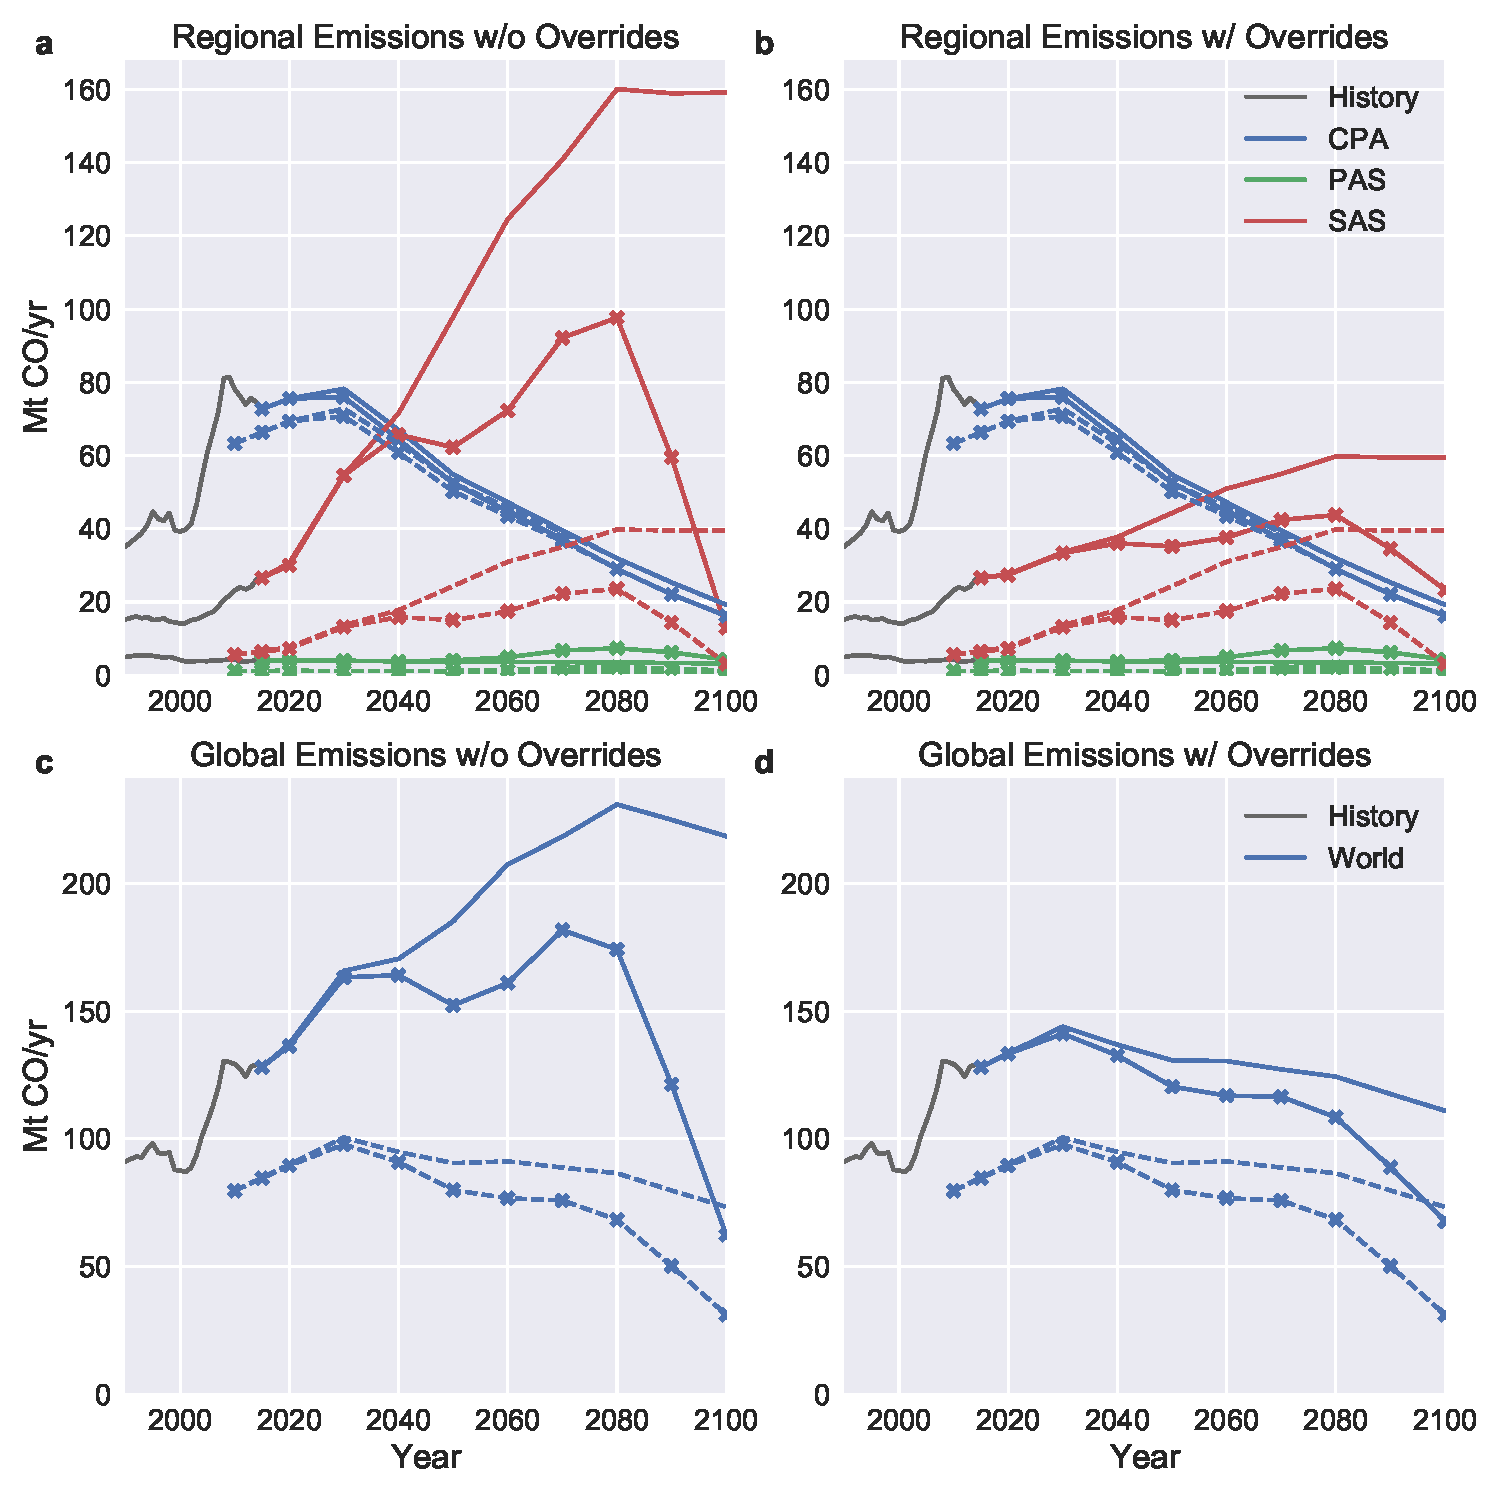
\includegraphics[width=\textwidth]{results_CO_Industrial_Sector.pdf}
    \caption[]{
      \label{fig:co}
      CO Industrial Sector harmonized and unharmonized emissions are presented
      for SSP2 and SSP2-45 scenarios. Scenarios as denoted identically to Figure
      \ref{fig:nox}. Panels \textbf{a} and \textbf{b} show harmonized and
      overridden-harmonized (respectively) regional trajectories for the 3
      MESSAGE-GLOBIOM regions that comprise the R5ASIA region: Centrally Planned
      Asia (CPA), Other Pacific Asia (PAS), and South Asia (SAS). Notably, the
      SAS regional trajectory displays a distorted trajectory due to the
      harmonization-year difference between history and model results in both
      scenarios. The distortion is large enough to affect global results, as
      shown in Panels \textbf{c} and \textbf{d}.  
}
  \end{center}
\end{figure}

In certain circumstances, the application of the default harmonization methods
can affect not only the magnitude but also the shape of regional
trajectories. Figure \ref{fig:nh3} shows an example case of emissions
trajectories for ammonia (\nht) from the agriculture sector in Asia. Again, the
SAS region shows a large discrepancy in the harmonization year ($>$150\% in this
case). The resulting trajectory harmonized with the default method
(\code{constant_ratio}) provides a large increase after 2080 in the SSP2
reference scenario. Notably, the SSP2-45 scenario is not affected to the same
degree. While this distortion changes the magnitude of the SAS trajectory, it
largely affects the post-2080 shape of the global trajectory (see Figure
\ref{fig:nh3}, panel \textbf{c}). By using a \code{constant_offset} method as an
override, this distortion is addressed and more accurately reflects unharmonized
results in the SAS region, the relative importance between regions, and global
results for agricultural ammonia emissions, each of which contributes to a
better harmonization quality for the harmonized SAS trajectory.

\begin{figure}
  \begin{center}
    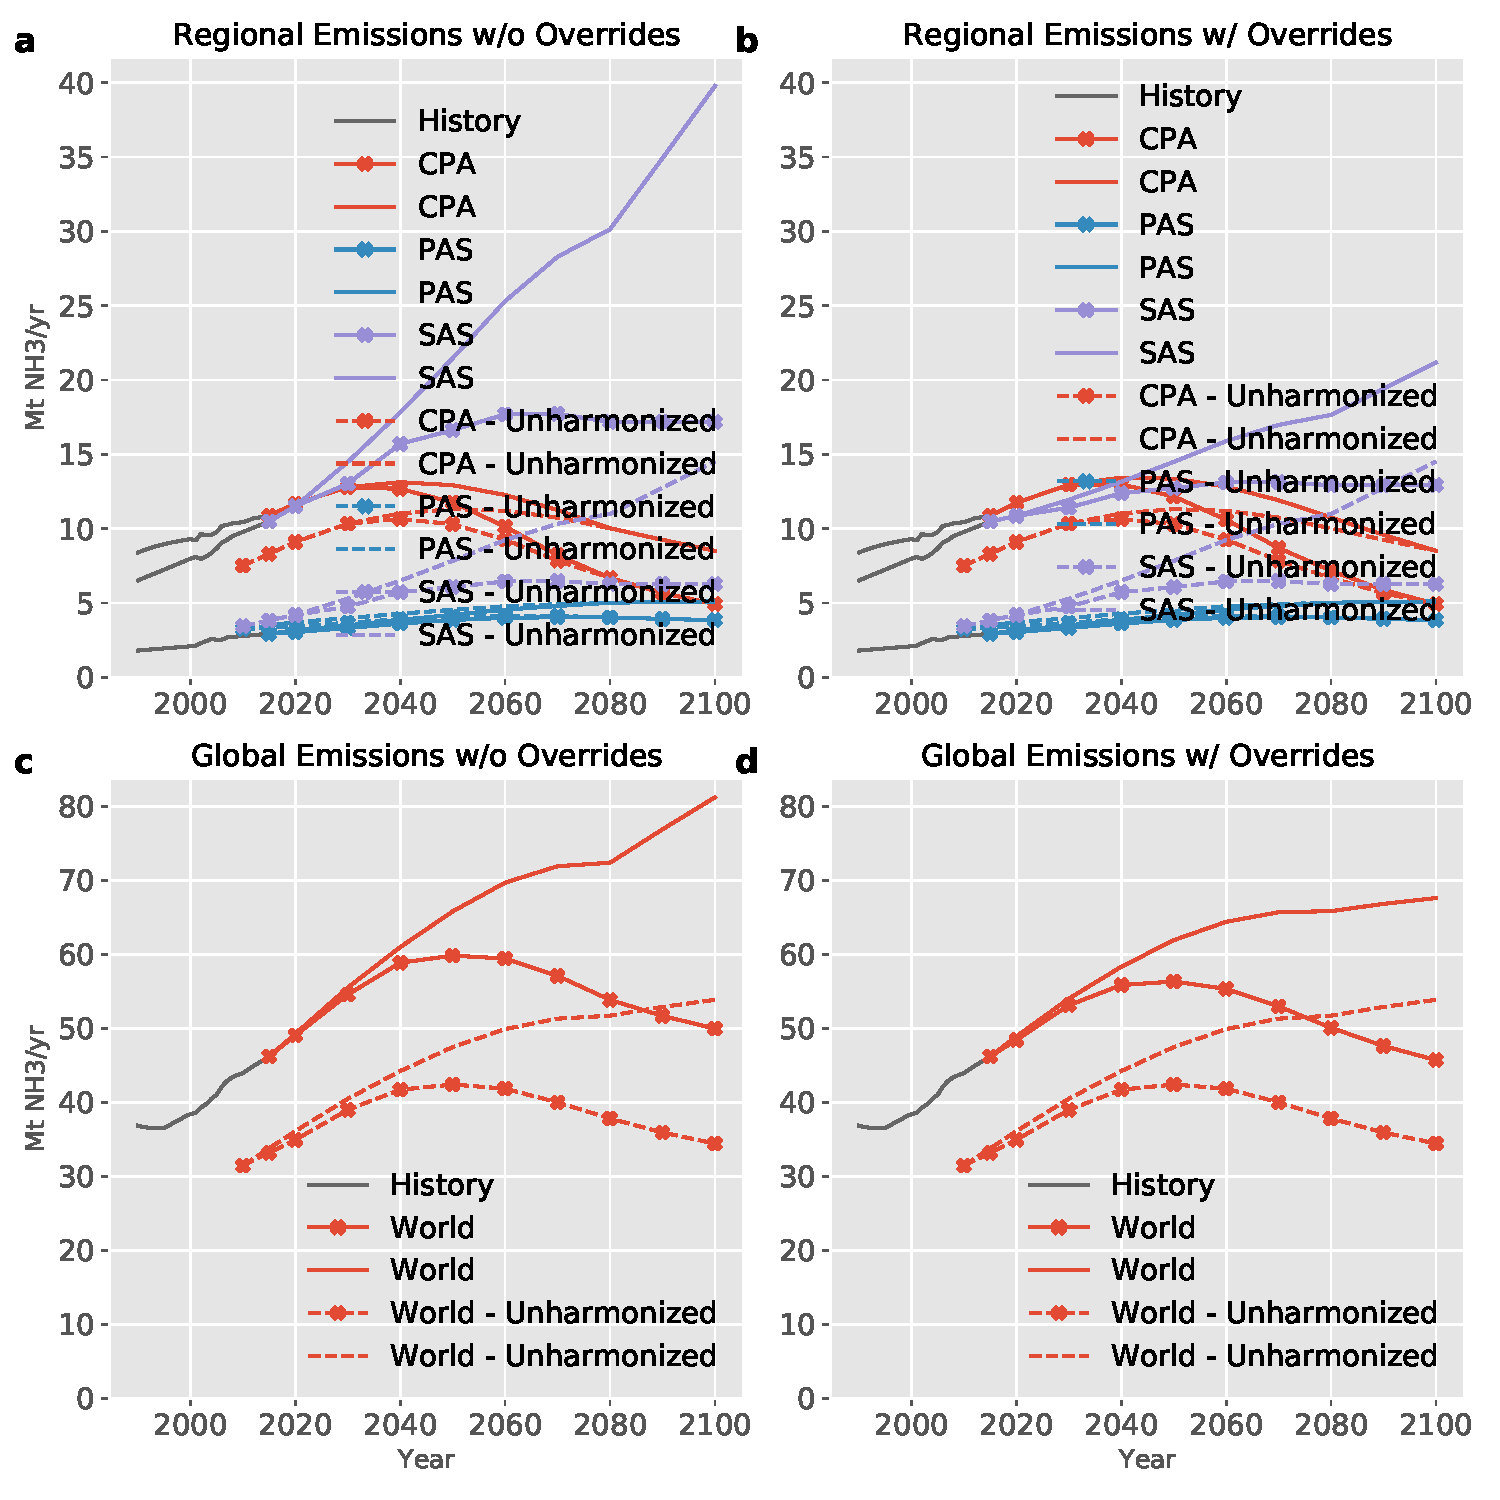
\includegraphics[width=\textwidth]{results_NH3_Agriculture.pdf}
    \caption[]{
      \label{fig:nh3}
      \nhtt agricultural harmonized and unharmonized emissions are presented for
      SSP2 and SSP2-45 scenarios. Scenarios and panel layouts are identical to
      Figure \ref{fig:co}. In this case, the SAS trajectory again shows not only
      a magnitude distortion, but also a shape distortion at the tail of the
      trajectory. Additionally, global trajectories are greatly affected by the
      harmonization method choice (there is $\sim$20\% relative difference
      between trajectories in the reference scenario in 2100). Override methods
      have been applied to correct the distortion.  }
  \end{center}
\end{figure}


We investigate the aggregate effect of harmonization with all necessary override
methods on total anthropogenic radiative forcing projections with the simple
carbon-cycle and climate model, MAGICC6 \cite{meinshausen2011emulating,
  meinshausen2011rcp}, for each harmonized and unharmonized scenario
respectively as shown in Figure \ref{fig:forcing}. We find that the change due
to harmonization is small, ranging between 1 and 2.5\% over the model
horizon. Relative near-term differences persist in the mitigation case (SSP-4.5)
because differences in near-term emissions define to a larger degree the
longer-term forcing outcome due to the cumulative nature of long-lived climate
forcers like \cotwo.  The resulting difference in forcing in 2100 is 0.04
$\frac{\text{W}}{\text{m}^2}$ for SSP2-4.5 and 0.01
$\frac{\text{W}}{\text{m}^2}$ for SSP2-Ref, both of which are well within
acceptable tolerances (e.g., 0.75 $\frac{\text{W}}{\text{m}^2}$ defined for
\gls{smip} \cite{oneill_scenario_2016}). Thus harmonization is considered to
have a negligible effect on key long-term climate indicators.

\begin{figure}
  \begin{center}
    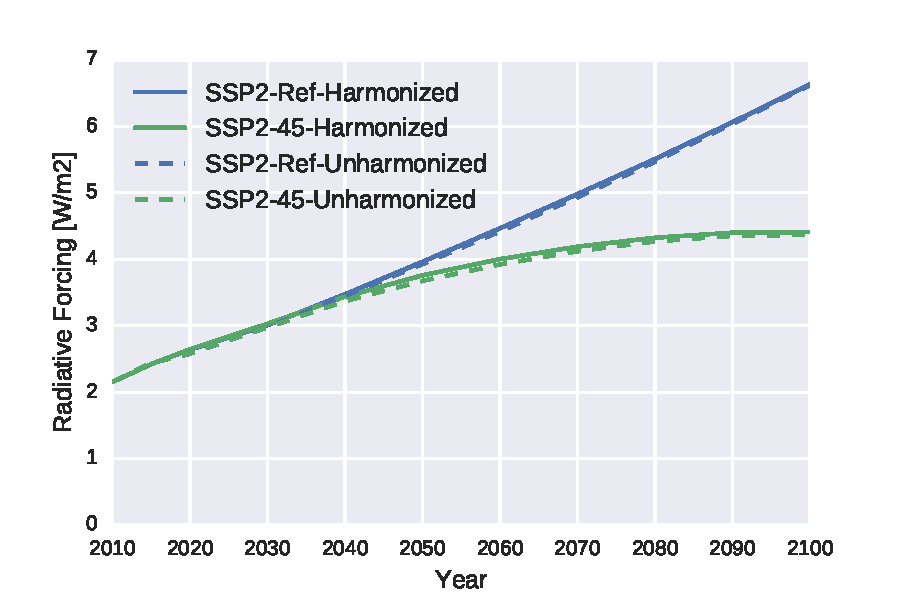
\includegraphics[width=\textwidth]{results_forcing.pdf}
    \caption[]{
      \label{fig:forcing}
      The results of the simple climate model, MAGICC6, forced with the SSP2-Ref
      (blue) and SSP2-4.5 (green) harmonized and unharmonized scenarios is
      presented. The radiative forcing trajectories of harmonized and
      unharmonized scenarios are shown in solid lines and dashed lines,
      respectively.  }
  \end{center}
\end{figure}
\section{Discussion \& Future Work}\label{sec:future}

This work presented a novel methodology and Python implementation of automated
emissions harmonization for \glspl{iam}, \code{aneris}. An in-depth explanation of the
processes and methods for determining the use of harmonization methods was
provided in Section \ref{sec:meths}. \code{aneris} was able to satisfactorily
harmonized over 96\% of the 1940 individual trajectories that were analyzed in
Section \ref{sec:results}. Of the remaining trajectories, harmonization method
overrides were applied, and example situations in overrides were needed were
discussed.

The automated approach drastically reduces the need for expert opinion in
determining harmonization methods for each individual combination of model
region, sector, and emissions species while still providing a justifiable
explanation for each automated choice of harmonization method based on both the
historical and future emissions trajectories. Furthermore, the automated
approach continues to scale well as models become more detailed in both the
regional and sectoral dimensions. Finally, expert opinion is still allowed to
trump the automated method as determined by the algorithm via method overrides;
however, these cases are clearly documented via the meta data provided as an
output of \code{aneris} and thus can be individually explained. This provides
not only transparency and reproducibility, but also scientific integrity in the
choice of harmonization methods.

The use of an open-source, automated harmonization process also provides
benefits to the wider climate science and \gls{iam} communities. By providing a
standard mechanism for harmonization, the \gls{iam} community can directly provide
input into the harmonization algorithms and rules for their default
selection. Additionally, modeling teams are easily capable of executing
identical harmonization procedures in order to participate in ongoing and
further iterations of intercomparison exercises and analysis. Future scenario
analyses can also utilize this common harmonization approach such that they are
consistent with prior efforts.

There are a variety of avenues for future improvement of both the \code{aneris}
software and underlying methodology. As with any software project, additional
users will provide use cases for more robust handling of input/output concerns
and corner cases. Further configuration parameters can also be added in the
future in order to provide overrides for all gas species in a given sector or
region. Perhaps the most fruitful investigation will involve further refinement
of the default decision tree introduced in Section \ref{sec:meths}. A key aspect
missing from the decision tree is input from models regarding whether missing
sources or activity levels are the likely cause of a harmonization year
discrepancy (suggesting the use of an offset method) or instead a significant
difference in emissions factors (suggesting the use of a ratio method)
\cite{rogelj_discrepancies_2011}.

This work provides a new direction and framework which the \gls{iam} and climate
communities can build upon in order to reduce the necessity of consistent expert
opinion and increase transparency and reproducibility of harmonization
exercises. Furthermore, it provides an open-source, tested, and documented
software library which can be used and improved upon by these communities. Both
of these are clear steps in a positive direction for future climate and
integrated assessment modeling exercises.

%%%%%%%%%%%%%%%%%%%%%%%%%%%%%%%%%%%%%%%%%%%%%%%%%%%%%%%%%%%%%%%%%%%%%%%%%%%%%%%%
\section*{Acknowledgements}

The authors would like to acknowledge a number of colleagues who helped
contribute both discussion and feedback regarding this work including Drs. Elmar
Kriegler, Gunnar Luderer, and Joeri Rogelj. This project has received funding
from the European Union’s Horizon 2020 research and innovation programme under
grant agreement No 641816. The authors further wish to thank the Global
Environment Facility for their generous financial support.

\newpage
%Print the glossary
\printglossaries

\newpage
\section*{\refname}
\bibliography{refs}
\end{document}
